\chapter{Az antik görög művészet}
\label{ch:2_antik_gorog}

\section{Az antik görög kor hitvilága, korszakai és építészete}

\tcbox[left=0mm,right=0mm,top=0mm,bottom=0mm,boxsep=0mm,
toptitle=0.5mm,bottomtitle=0.5mm,title=\centering{A tétel adatai}]{%
	
	\begin{tabular}{| p{0.25\textwidth} | p{0.75\textwidth} |}		
		\hline
		Tétel teljes címe & Mutassa be az antik görög kor hitvilágát, korszakait és építészetét! Elemezze a legismertebb épületeit, művészeti alkotásait!
		\\ \hline
		
		Jegyzetek &
		\begin{compactitem}
			\item Az ókori görög művészet és kultúra korszakai, jellemzői.
			\item A templomok felépítése, az oszloprendek jellemzői.
			\item A görög szobrászat jellegzetes vonásai a különböző korszakokban.
			\item A görög mitológia világa, a görög vázafestészet.
		\end{compactitem}
		\\\hline
		
	\end{tabular}}

\clearpage

\subsection*{Hitvilág}

\paragraph{Nem egységes} 
Egy igen bonyolult és ellentmondásoktól sem mentes görög világ vallását szoktuk leegyszerűsítve görög vallásnak nevezni. A görög föld nem volt egységes, nem is alakult ki egységes papi testület. A vallás összefonódott a városállammal.

\paragraph{Istenek}
A görögök sokistenhívők voltak: számos istent tiszteltek (politeizmus), melyeket emberi alakkal és tulajdonságokkal ruháztak fel (antropomorfizmus). Az istenek lakóhelyének Görögország legmagasabb hegyét, a Thesszália északi részében álló Olümposzt tartották. Itt élnek örökös derű közepette, Zeusz uralma alatt; alakjuk, sőt jellemvonásaik és vágyaik is az emberéihez hasonlók, csak szebbek, nagyobbak és erősebbek, s halhatatlanság és örök ifjúság az osztályrészük.

\paragraph{Mitológia}
Az istenek kalandos élete, viszontagságai, harcai, szerelmei a görög mítoszokban jelentek meg. A görög mitológia színes, költői leírásokban beszél erről, továbbá a világ és az emberiség keletkezéséről és ősi történetéről.

\paragraph{Jelentősebb istenek}
\begin{compactitem}
	\item \textbf{Zeusz} - Olümposzi legfőbb isten, az „emberek és istenek atyja”, az ég és a villámok ura. 
	
	\item \textbf{Hádész} - Az alvilág istene, a holtak ura.
	
	\item \textbf{Héra} -  Zeusz főisten testvére és felesége, a házasságot és a születést védelmező istennő.
	
	\item \textbf{Dionüszosz} - A bor és mámor megtestesítője, aki értett a mezőgazdasághoz és termékenységet is hozhatott. Ő volt a görög színjátszás patrónusa is.
	
	\item \textbf{Apollón} -  Zeusz és Létó gyermeke, Artemisz ikertestvére. A költészet, a jóslás, a zene, a tánc, a művészetek, a férfi szépség, a fény, az íjászat és a gyarmatosítás istene.
	
	\item \textbf{Héphaisztosz} - A kovácsmesterség, a tűz istene a görög mitológiában. Védelmezője minden mesterembernek, főként a fémműveseknek. A vulkánok istenét is tisztelték benne. 
	
	\item \textbf{Aphrodité} - A szerelem és a szépség istennője. 
	
	\item Athéné - Pallasz Athéné a bölcsesség, az igazságos háború, a jog, az igazságosság, a művészetek, a kézművesség és a képzés istennője.
	
	\item Hermész -  Zeusz és Maia nimfa gyermeke, az istenek hírnöke a görög mitológiában.
	
	\item Árész - A háború istene, Zeusz és Héra gyermeke. Pallasz Athénével ellentétben nem bölcsen vezetett hadat és ezért nem a győzedelmes és igazságos háború, küzdelem istene volt, hanem az értelmetlen vérontás és kegyetlen öldöklés megtestesítője.
	
	\item Artemisz -  Zeusz és Létó gyermeke, Apollón ikertestvére a görög mitológiában. A Hold és a vadászat szűz istennője, ő segít a szülésnél és védelmezi a nőket és a gyermekeket. A vadállatok úrnője is.
	
	\item Démétér - A földművelés és a termékenység istennője.
\end{compactitem}

\vspace{0.5cm}

\begin{tcolorbox}[enhanced,colframe=gray!50!white,
	colbacktitle=white!15!white,
	coltitle=gray!50!black,
	borderline={0.5mm}{0mm}{gray!15!white},
	borderline={0.5mm}{0mm}{gray!50!white,dashed},
	attach boxed title to top center={yshift=-2mm},
	boxed title style={boxrule=0.4pt},
	title=Görög istenek]{
	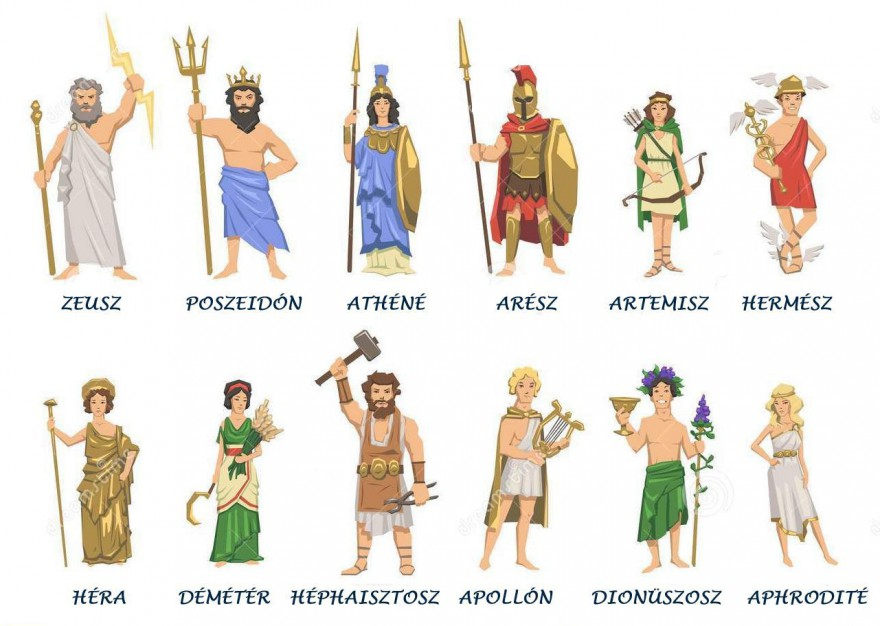
\includegraphics[width=1.0\linewidth]{02/gorog_istenek}}
\end{tcolorbox}

\subsection*{Korszakok}

\tcbox[left=0mm,right=0mm,top=0mm,bottom=0mm,boxsep=0mm,
toptitle=0.5mm,bottomtitle=0.5mm,title=\centering{Az ókori Görögoszág korszakai}]{%
	
	\begin{tabular}{| p{0.1\textwidth}|p{0.1\textwidth} | p{0.75\textwidth} |}
		
		\centering{\textbf{Homé- roszi kor}}
		&
		i. e. XII - VIII. sz.
		&
		A görög sötét kor (kb. i. e. 1200–i. e. 800) Görögország történetének a feltételezett dór vándorlás kezdetétől és a mükénéi civilizáció i. e. 11. századi végétől az első görög városállamoknak – poliszoknak – az i. e. 9. századi felemelkedéséig, a homéroszi epika és a görög ábécé i. e. 8. századi megjelenéséig tartó időszaka.
		\\\hline
		
		\centering{\textbf{Archai- kus kor}}
		&
		i. e. VII - VI. sz.
		&
		Kialakul a görög templomtípus, a ión és a dór oszlopok. A szobrászat a valláshoz kapcsolódik: a szobrok sírokból kerültek elő. Két típusuk a kúrosz (mezten férfi szobor) és kóré (egyszerű drapériába öltözött női alak). A vázafestészetre jellemző három stílus a geometrikus, orientalizáló és fekete alakos.
		\\\hline
		
		\centering{\textbf{Klasz- szikus kor}}
		&
		i. e. V - IV. sz.
		&
		A kor központja Athén. Az athéni akropolisz leghíresebb épülete a Parthenon, Athéné Parthenosz (=Városvédő Athéné) temploma. Kialakul a görög színház. A szobrászat három korszaka a korai, szigorú stílus, az érett és a késő klasszikus kor. A korai és érett szakasz témája a sportos, idealizált, izmos, tettre és harcra kész férfi (példák az érett korszakból: Polükleitosz: Dárdavivő, Müron: Diszkoszvető, Pheidiász: Athéné Parthenosz). Az érett korban megjelenik a kontraposzt tartás, mely Polükleitosz nevéhez fűződik. A késői korszak célja inkább a gyönyörködtetés és az érzelmek megragadása, ezért kisebb hangsúlyt kap az izmok aprólékos kidolgozása (pl. Praxitelész: Hermész a kis Dionüszosszal, Knidoszi Aphrodité). Megjelenik a vörösalakos stílus a vázafestészetben.
		\\\hline
		
		\centering{\textbf{Helle- nizmus kora}}
		&
		i. e. IV - II. sz.
		&
		A hellenizmusban Nagy Sándor (Alexandrosz) hódításai okán a városépítészet kerül a középpontba. A szobrászat témája a mindennapi valóság reális, naturalisztikus ábrázolása, középpontjában az ember van.
		\\\hline
\end{tabular}}

\clearpage

\subsection*{Homéroszi kor}

A görög sötét kor (kb. i. e. 1200 – i. e. 800) kifejezés azt a korszakot jelenti a görög történelemben, ami a feltételezett dór invázióval, a mükénéi civilizáció bukásával kezdődött és az első görög városállamok i. e. 9. századi, valamint Homérosz epikájának és a görög alfabetikus írás i. e. 8. századi megjelenéséig tartott.

Úgy tartják, Homérosz epikája tartalmaz bizonyos mennyiségű, a sötét korból eredő szájhagyományt. Homérosz írásainak történeti helyessége erősen vitatott.

Ezt a kort előzte meg az égei kultúra.

\subsubsection{A homéroszi kort megelőző égei kultúra és mondaköre}

\begin{wrapfigure}{r}{0.65\textwidth}
	\tcbox[colback=darkgray!85!black,
	left=0mm,right=0mm,top=0mm,bottom=0mm,boxsep=1mm,toptitle=0.5mm,bottomtitle=0.5mm,
	title=\centering{Az égei kultúra földrajzi helyszínei}]{
		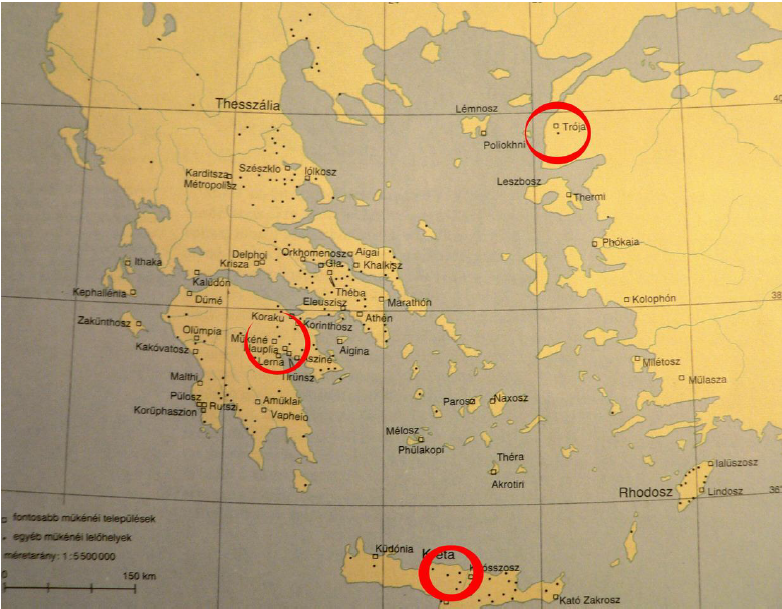
\includegraphics[width=1.0\linewidth]{02/mukene}
	}
\end{wrapfigure}
Az Égei tenger medencéjében és Kréta szigetén élő nép, az égei civilizáció volt a görögök elődje.

A mükénéi kultúra a görög szárazföld késő bronzkori kultúrája (Kr. e. 16–12. sz.). Nevét egyik legjelentősebb lelőhelyéről, Mükénéről kapta. Rajta kívül fontos központok és lelőhelyek voltak Pülosz, Spárta és Tirünsz is. Egy időbe esik az égei kultúrával (Kréta szigete, Knósszoszi palota) és a Tórjai mondakör idejével.

\paragraph{Trójai mondakör}
Agamemnon mükéné királya szövetségbe kényszerítette a görög királyságokat egyedül Thesszália maradt független, Agamemnon öccse Menelaosz a Spártai király belefáradt a háborúba és békét akart kötni Trójával a megerősödött görögök legnagyobb riválisával. A békekötés ünnepén ismerkedett össze Páris Szép Helenével, Menelaosz feleségével, akit távozásukkor magával vitt Trójába. Agamemnont kérte meg Menelaosz hogy segítsen visszaszerezni felségét, akinek ez jó ürügy volt Trója meghódítására. Agamemnon legjobb és leghíresebb mitológiában is szereplő harcosa Akhilleusz is velük tartott, legjobb barátjával Patroklosszal együtt. A Trójai ifjúk (Hektor és öccse Páris) harcba szálltak Agamemnon seregeivel. A csata 10 évig tartott. Akhilleusz a Parisz képében megjelent Apollón sarkába lőtt nyílvesszőjétől halt meg (Akhilleusz félisten volt, egyetlen sebezhető pontja a sarka volt, mivel mikor anyja a Sztüx vizébe mártotta, hogy sérthetetlenné tegye az kilógott a folyóból).

Trója akkor bukott el mikor egy csellel a görögök látszat visszavonulást hajtottak végre, és ajándékba egy falovat adtak, amit ők az isteneknek szánt ajándék gyanánt bevontattak a városba. Azonban este az ünnep alatt görög katonák másztak elő a falóból, és kinyitották Trója bevehetetlen városának kapuit a visszaérkező görög seregnek. Ekkor esett el Trója.

\paragraph{A Knószoszi palota mitológiája}
A Krétai király, Minosz Poszeidón segítségével nyerte el a hatalmat, azoban megfeledkezett az istennek ígért áldozatról. Ezért Poszeidón egy bikát küld a városra a tengerből, aki frigyre kel Minosz feleségével. A nász következménye a bika fejű, ember testű lény, a minotaurosz. Minosz szégyenében elrejti őt egy labirintusba.

Amikor lánya, Ariadné kerül sorra a minotaurosznak szánt áldozatok között, Thészeusz megöli a minotauroszt és Ariadné fonalának segítségével kijut a labirintusból.

A labirintust Knószosz palotájával szokás azonosítani, mivel annak alaprajza bonyolult, labirintusszerű.

\paragraph{A mükénéi akropolisz}
Ez a legősibb, legrégebbi polisz a Peloponészoszi - félszigeten. A várost műkénéi akropolisznak nevezték el, mert a város egy magaslaton található erődítményszerű falakkal körülvéve. Az uralkodói palota, temetkezési hely és vallásos célú építmények is találhatók a poliszban. Heinrich Schliemann fedezte fe majd tárta fel.

\clearpage

\subsection*{Archaikus kor}

Ebben az időben alakul ki az a görög templomtípus, amely máig az építészettörténetben kifejti hatását, akkor alakulnak ki a görög oszloprendek, a különböző alaprajzi típusok.

\subsubsection{A görög templom}

\begin{wrapfigure}{r}{0.35\textwidth}
	\begin{tcolorbox}[enhanced,colframe=gray!50!white,
		colbacktitle=white!15!white,
		coltitle=gray!50!black,
		borderline={0.5mm}{0mm}{gray!15!white},
		borderline={0.5mm}{0mm}{gray!50!white,dashed},
		attach boxed title to top center={yshift=-2mm},
		boxed title style={boxrule=0.4pt},
		title=Dór és ión oszlop]{
		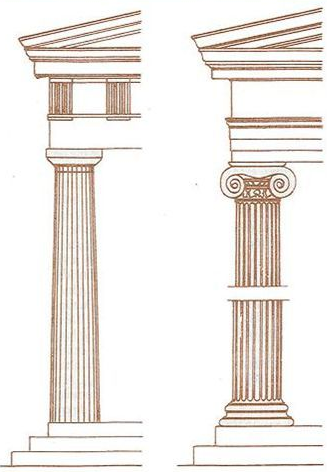
\includegraphics[width=1.0\linewidth]{02/dor_ion_oszlop}}
	\end{tcolorbox}
\end{wrapfigure}

Az archaikus korra elsősorban templommaradványok utalnak. A korai faoszlopos, agyag falú, kőalapozású templomokat kőépületek váltották fel. Fokozatosan kialakultak az oszloprendek, a dór és az ión oszlopokkal, az előbbi a férfi, az utóbbi a női test arányait követte. A templomok oromzatát, a timpanonokat domborművek díszítették, a falakat pedig frízek.

Az antik templom álltalában magaslaton, zöld környezetben állt, harmonizált a természettel és óriási gonddal, művészi kivitelben készültek.

\begin{wrapfigure}{r}{0.4\textwidth}
	\tcbox[colback=darkgray!85!black,
	left=0mm,right=0mm,top=0mm,bottom=0mm,boxsep=1mm,toptitle=0.5mm,bottomtitle=0.5mm,
	title=\centering{Héra temploma Olümpiában}]{
		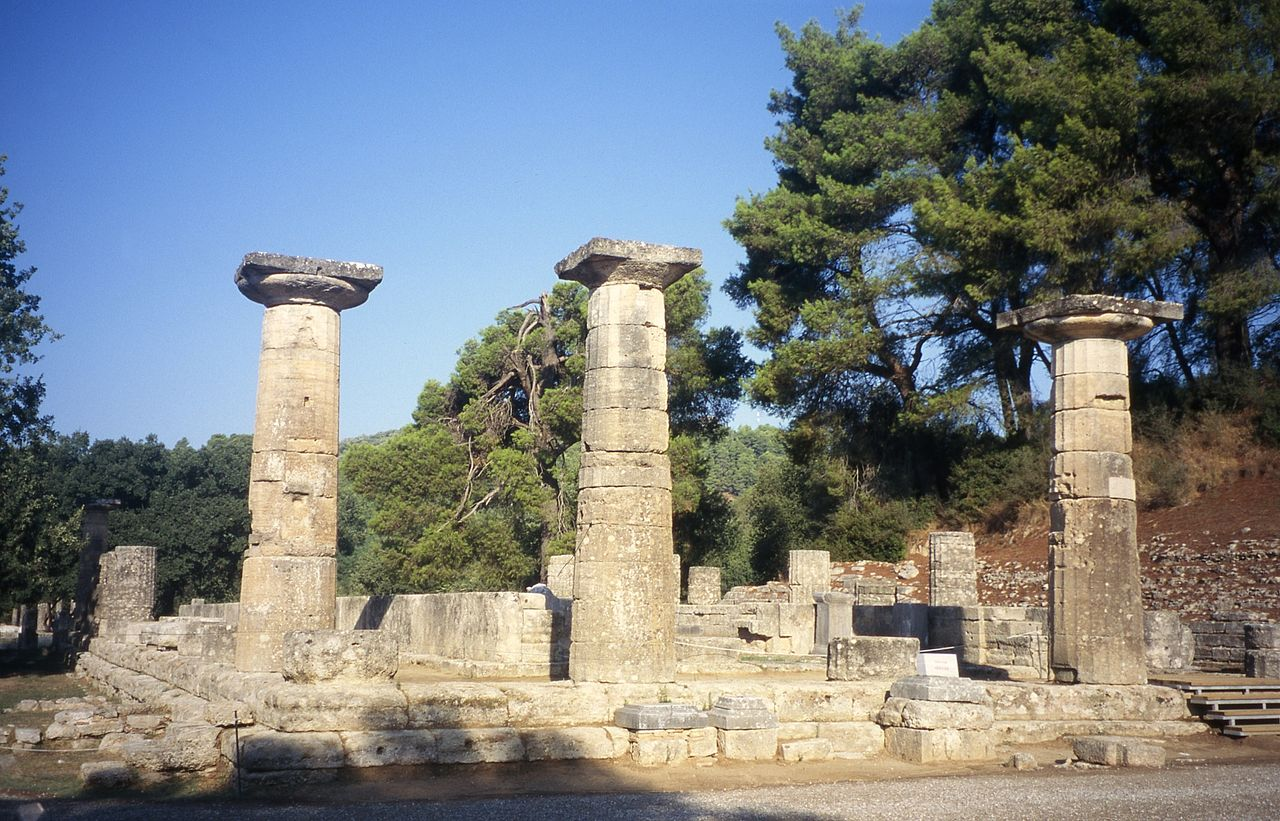
\includegraphics[width=1.0\linewidth]{02/hera_templom}
	}
\end{wrapfigure}

\paragraph{Tájolás}
A templom tájolása kelet-nyugati, bejárata kelet felé néz, hogy a felkelő nap a bejárattal szemben lévő isten szobrot világítsa meg.

\paragraph{Rendeltetés} A templomnak nem alkalmasak arra, és nem céljuk, hogy nagy tömegeket fogadjanak be, a nyilvános szertartások a templom előtt zajlottak és nem a templomban. Az épületbe csak a papok mehettek be. Az épület célja, hogy a benne álló görög istenség szobrát és oltárát, valamint az adományokat és kincseket megvédje, megőrizze akár az időjárástól, akár az illetéktelen személyektől és méltóságteljes építészeti keretet adjon azoknak.

\begin{wrapfigure}{r}{0.45\textwidth}
	\tcbox[colback=darkgray!85!black,
	left=0mm,right=0mm,top=0mm,bottom=0mm,boxsep=1mm,toptitle=0.5mm,bottomtitle=0.5mm,
	title=\centering{Az antik templom típusai}]{
		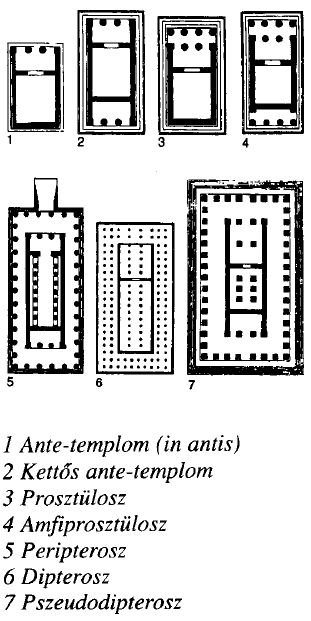
\includegraphics[width=1.0\linewidth]{02/antik_templom_tipusai}
	}
\end{wrapfigure}

Az építtetők maguk a polgárok és vezetőik, az építészek neve legfeljebb a mitológiában maradnak fönn.

\paragraph{Típusok}

\subparagraph{Megaron} Az első alaprajz neve a Megaron volt. A megaron az ősi görög lakóház egyszerű formáját követi, oszlopok nélküli téglalap alakú tér.

\subparagraph{Ante-templom} A második az Ante-templom, amihez Kelet felől a bejáratnál két falpillér alkot előcsarnokot , amihez két oszlop is kapcsolódott.

\subparagraph{Peripterosz} Leggyakoribb alaprajzi típus, ahol a tégla alaprajzú fal minden oldalán oszlopsor fut körbe.

\vspace{2cm}

\begin{figure}[!h]
	\begin{tcolorbox}[enhanced,colframe=gray!50!white,
		colbacktitle=white!15!white,
		coltitle=gray!50!black,
		borderline={0.5mm}{0mm}{gray!15!white},
		borderline={0.5mm}{0mm}{gray!50!white,dashed},
		attach boxed title to top center={yshift=-2mm},
		boxed title style={boxrule=0.4pt},
		title=A görög templom részei]{
			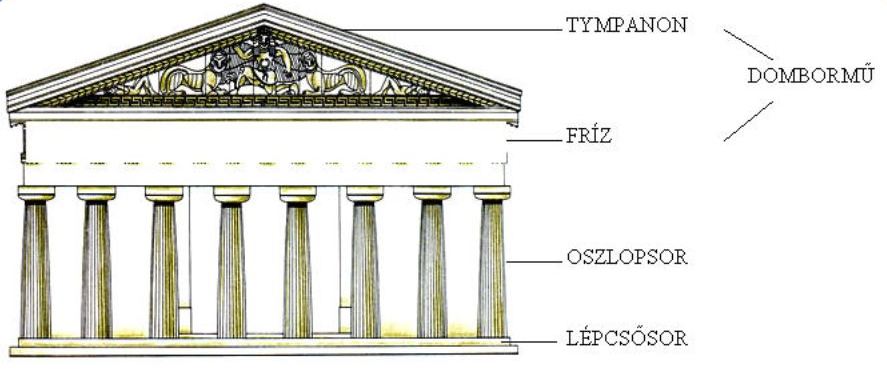
\includegraphics[width=1.0\linewidth]{02/templom_reszei}}
	\end{tcolorbox}
	\captionsetup{labelformat=empty}
	\caption{}
\end{figure}

\clearpage

\subsubsection{Szobrászat}

\begin{wrapfigure}{r}{0.3\textwidth}
	\begin{minipage}{0.3\textwidth}
		\tcbox[colback=darkgray!85!black,
		left=0mm,right=0mm,top=0mm,bottom=0mm,boxsep=1mm,toptitle=0.5mm,bottomtitle=0.5mm,
		title=\centering{Kúrosz}]{
			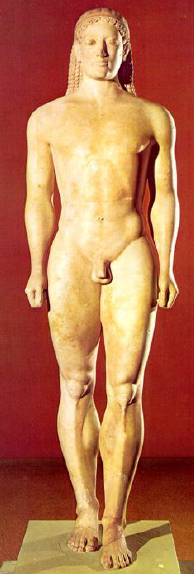
\includegraphics[width=1.0\linewidth]{02/kurosz}
		}		
	\end{minipage}
	\begin{minipage}{0.3\textwidth}		
		\begin{tcolorbox}[enhanced,colframe=gray!50!white,
			colbacktitle=white!15!white,
			coltitle=gray!50!black,
			borderline={0.5mm}{0mm}{gray!15!white},
			borderline={0.5mm}{0mm}{gray!50!white,dashed},
			attach boxed title to top center={yshift=-2mm},
			boxed title style={boxrule=0.4pt},
			title=Kóré]{
				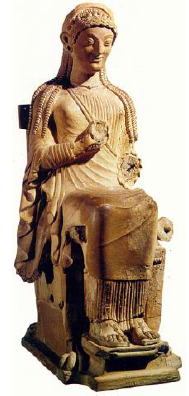
\includegraphics[width=1.0\linewidth]{02/kore}}
		\end{tcolorbox}	
	\end{minipage}
\end{wrapfigure}

Az antik archaikus szobrok a \textbf{valláshoz kapcsolódnak} (temetkezési, fogadkozási szobrok). Sírokban találták meg őket valamint úgy nevezett a görög isteneknek segítségkérés gyanánt ajánlják fel, a templomok kincstáraiban maradtak fenn.

Két típus alakult ki: a \textbf{kúrosz} (ruhátlan férfialak) és a \textbf{kóré} (ruhás nőalak). A fáraó-szobrokhoz hasonlítanak leginkább zárt tömegkezelés volt rájuk jellemző.

\paragraph{Kúrosz jellemzői} A kúroszra tömbszerű kompozíció, frontális beállítás volt jellemző: (arc, törzs, láb, szembenéz) kezek szorosan a comb mellett, bal láb előrelép, statikus, merev, idealizált, fiatal, „szép” arc, archaikus mosoly (érzelem, öröm kifejeződése) aprólékos csigás haj. A fő különbség a fáraó szobroktól: az izomzat akár stilizáltan, akár reálisan, de mindenképp részletesebben bemutatva jelenik meg

\paragraph{Kóré jellemzői} Kóré jellemzése: monoton, egy forma „függőleges” sűrűn redőzött,
drapéria, nincs benne mozgás, nincs benne variáció, nem bonyolult és kezével apró mozdulatot tesz.

\subsubsection{Vázafestészet}

A vázafestészetben három stílust különböztetünk meg: geometrikus, orientalizáló, fekete alakos.

\paragraph{Geometrikus stílus}
Geometrikus, mértani formák jelennek meg a vázán.

\clearpage 

A vörös alapfelület a fedetlen terrakotta és erre kerül rá fekete mázzal a díszítmény vízszintes vonalakban.

\paragraph{Orientalizáló stílus}
A vázán megjelenő motívumok a keleti területek hatását tükrözik jellemzői a geometrikus motívumokat fölváltják a hullámzó motívumok, díszítmények és emellett az állatfigurák kapnak főszerepet.

\paragraph{Fekete alakos stílus}
Terrakotta alapon a figurák fekete mázzal vannak festve, de bennük már a részletek is ábrázoltak, méghozzá úgy, hogy a vonalakat belekarcolják a fekete mázba.

\begin{figure}[!h]
	\begin{minipage}{0.23\textwidth}
		\tcbox[colback=darkgray!85!black,
		left=0mm,right=0mm,top=0mm,bottom=0mm,boxsep=1mm,toptitle=0.5mm,bottomtitle=0.5mm,
		title=\centering{Geometrikus stílusú váza}]{
			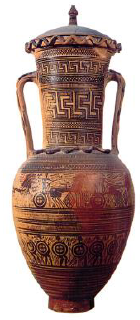
\includegraphics[width=1.0\linewidth]{02/geometrikus_vaza}
		}
	\end{minipage}
	\hfill
	\begin{minipage}{0.33\textwidth}
		\tcbox[colback=darkgray!85!black,
		left=0mm,right=0mm,top=0mm,bottom=0mm,boxsep=1mm,toptitle=0.5mm,bottomtitle=0.5mm,
		title=\centering{Orientalizáló stílusú váza}]{
			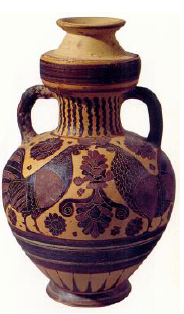
\includegraphics[width=1.0\linewidth]{02/orientalizalo_vaza}
		}
	\end{minipage}	
	\hfill
	\begin{minipage}{0.39\textwidth}
		\tcbox[colback=darkgray!85!black,
		left=0mm,right=0mm,top=0mm,bottom=0mm,boxsep=1mm,toptitle=0.5mm,bottomtitle=0.5mm,
		title=\centering{Fekete alakos váza}]{
			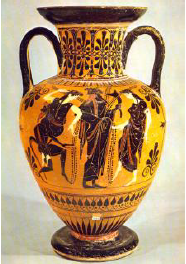
\includegraphics[width=1.0\linewidth]{02/fekete_alakos_vaza}}
	\end{minipage}
	\captionsetup{labelformat=empty}
	\caption{}
\end{figure}

\newpage


\subsection*{Klasszikus kor}

A klasszikus kor a görög művészet virágkora a Kr.e. V-IV. században (Kr.e.333, azaz Nagy Sándor fellépéséig – Nagy Sándorral kezdődik a hellenizmus). Három periódusra osztható korai klasszikus kor, érett klasszikus kor (a klasszikus kori művészet csúcsa, Kr.e. 450-430 között) késő-klasszikus kor.

A klasszikus kor a görög történelem legjelentősebb korszakában alakult ki, nem véletlen, hogy szinte minden későbbi művészettörténeti stíluskorszakra hatással volt.

\paragraph{Filozófia} Ebben a korban meginogtak a vallási hagyományok, az istenek tekintélyének szigora, a figyelem középpontjába a fizikai valóság került. Az ember saját kilétéről tett fel kérdéseket, saját maga és léte került gondolkodásának középpontjába (így születik meg a filozófia). Ez a szemlélet érvényesül a művészetben is: a művészetek fő témája az ember lett.

\begin{wrapfigure}{r}{0.45\textwidth}
	\tcbox[colback=darkgray!85!black,
	left=0mm,right=0mm,top=0mm,bottom=0mm,boxsep=1mm,toptitle=0.5mm,bottomtitle=0.5mm,
	title=\centering{Az athéni Akropolisz}]{
		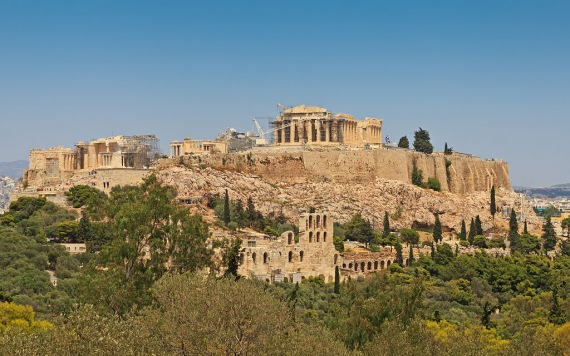
\includegraphics[width=1.0\linewidth]{02/athen}}
\end{wrapfigure}

\paragraph{Politika} 
A klasszikus kor \textbf{központja Athén}. A jólétet biztosító demokratikus poliszban megváltozik a művészet megítélése – a művészet nem a vallás kiszolgálója többé, hanem az állami reprezentáció, a politika eszköze. A legjelentősebb megrendelővé az állam, azaz a polisz, ill. annak vezetősége válik, valamint a nagypolgárság.

Az épületek számára gazdag szobrászati díszt rendelnek, így a városba özönlenek a művészek a félsziget minden területéről, és Athén a görög művészet központjává válik.

A demokráciában megváltozik a művészek megítélése is: míg korábban a művészek ahhoz a kézműves réteghez tartoztak, akiknek polgárjoguk sem volt, most a megtisztelt, szavazati joggal rendelkező athéni polgárság tagjai lesznek. Jól érzékelteti a művészek társadalmi rangjának megváltozását, hogy az alkotók nevei egyedül ebből a görög korszakból maradtak fenn.

\subsubsection{Építészet}

\begin{wrapfigure}{r}{0.45\textwidth}
	\tcbox[colback=darkgray!85!black,
	left=0mm,right=0mm,top=0mm,bottom=0mm,boxsep=1mm,toptitle=0.5mm,bottomtitle=0.5mm,
	title=\centering{Epidauroszi színház}]{
		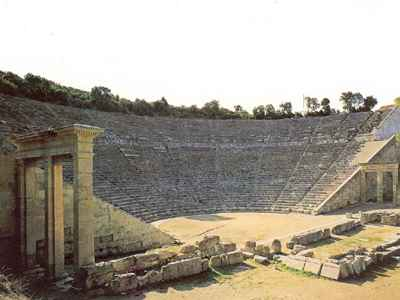
\includegraphics[width=1.0\linewidth]{02/epidauroszi_szinhaz}}
\end{wrapfigure}

\paragraph{Színház}
A görög színház Dionüszosz, a bor istenének ünnepein előadott paraszti játékokból alakult ki. A színház az akropoliszokon található Dionüszosz templom közelébe, a hegyoldal jó akusztikájának köszönhetően a hegy természetes módon körülölelő terébe került. Az egész fedetlen volt.

A színházépület négy részből áll: orkesztra \textit{(színház központja, kör alakú tér, a kórus helye)}, theátron \textit{(lépcsőzetes, hegyoldalba kialakított nézőtér)}, színpad \textit{(az orkesztra nézőtérrel átellens oldalán, itt játszottak a színészek)}, szkéné \textit{(színpad mögötti színfal, díszletként és takarásként szolgált, egyetlen felépítmény)}.

A leghíresebb, legjobb állapotban fennmaradt színház a 14 ezres tömegbefogadásra képes Epidauroszi színház volt. (Epidaurosz jelentős volt, Aszklépiosznak, a gyógyítás istenének kultuszhelye volt.)



\paragraph{Tholosz}
Olyan kör alaprajzú templom, amelyet oszlopsor vesz körül, és lépcsős alépítményen áll (akár a legtöbb  görög templom). Belső tere álltalában osztatlan. Leghíresebb példája szintén Epidauroszban van, az Epidauroszi kerek templom.

\paragraph{Az athéni Akropolisz}
Az akropolisz (görögül: felsőváros) az ókori görög városállamok általában magaslaton, hegytetőn épült fellegvára volt. Itt állt a királyi palota és a város védőistenének temploma, ezért idővel a városállam vallási központja lett. Leghíresebb az athéni akropolisz.

\paragraph{Az athéni Parthenon}

Az akropolisz fő épülete, méreteit tekintve a legnagyobb (kb.31x70 m területű) az itt található templomok között, elhelyezkedésében is a legmagasabban áll, anyaghasználatában is igényes és nemes: a templom márványból épült.

A templom Athéné Parthenosz, azaz a Városvédő Athéné istennő számára készült, a naoszban az istennő hatalmas szobra állt.


\begin{wrapfigure}{r}{0.45\textwidth}
	\centering
	\begin{minipage}{0.45\textwidth}
		\tcbox[colback=darkgray!85!black,
		left=0mm,right=0mm,top=0mm,bottom=0mm,boxsep=1mm,toptitle=0.5mm,bottomtitle=0.5mm,
		title=\centering{A Parthenon alaprajza}]{
			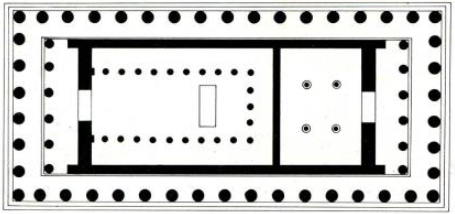
\includegraphics[width=1.0\linewidth]{02/parthenon_alaprajz}}
	\end{minipage}

	\begin{minipage}{0.45\textwidth}
		\tcbox[colback=darkgray!85!black,
		left=0mm,right=0mm,top=0mm,bottom=0mm,boxsep=1mm,toptitle=0.5mm,bottomtitle=0.5mm,
		title=\centering{Parthenon belsejének rekonstrukciója}]{
			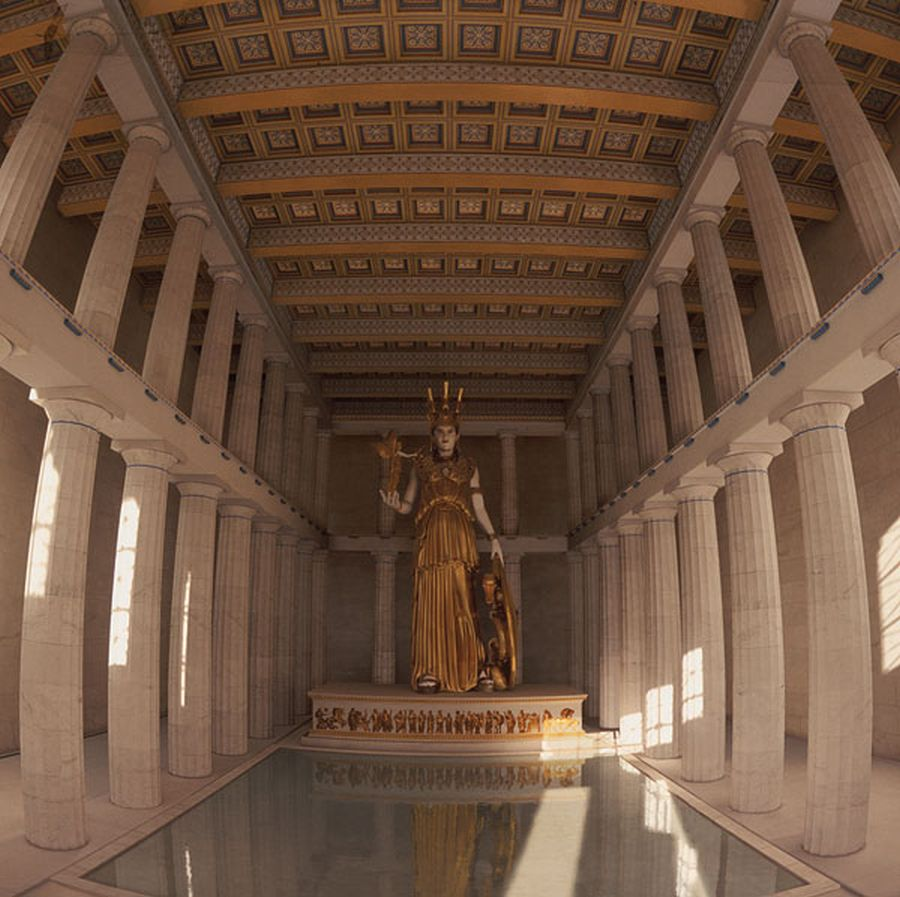
\includegraphics[width=1.0\linewidth]{02/parthenon_belseje}}
	\end{minipage}

	\begin{minipage}{0.45\textwidth}
		\tcbox[colback=darkgray!85!black,
		left=0mm,right=0mm,top=0mm,bottom=0mm,boxsep=1mm,toptitle=0.5mm,bottomtitle=0.5mm,
		title=\centering{Az athéni parthenon}]{
			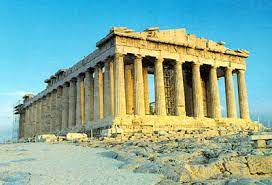
\includegraphics[width=1.0\linewidth]{02/parthenon}}
	\end{minipage}
\end{wrapfigure}
\subparagraph{Alaprajza}
Az archaikus korban kialakult peripterosz elrendezést követi: hosszanti, téglalap alakú falait minden oldalról oszlopok veszik körül.

Az épületet körülvevő oszlopsoron belül a templom mindkét rövidebbik oldalán a bejáratok előtt egy-egy oszlopos előcsarnok is van.

A belső két részre oszlik: a keleti oldalról nyíló nagyobb térre, a naoszra, ahol az istennő szobra és oltára állt, és egy kisebb térre a nyugati oldalon, ami valószínű, hogy kincstárként szolgált.

\subparagraph{Belső}
A belső legfőbb dísze a hatalmas szobor és az azt körülvevő oszlopsor volt. Az oszlopsor különlegessége abban rejlett, hogy kétszintes volt: egy masszívabb dór oszlopsor egy kisebb szintén dór oszlopsort tartott. Így az épület kelet-nyugati tájolásának köszönhetően a keleti bejárat felől a reggeli napfény a szobrot világította meg.

\subparagraph{Térlefedés}
Nyitott fa fedélszékkel volt fedve a templom (ebből természetesen mára már semmi nem maradt meg), ennek súlyát tartották az oszlopsorok és falak.

\clearpage

\subparagraph{Külső}
Az épület a hírnevét a monumentális, tekintélyt parancsoló, ugyanakkor harmonikus, kiegyensúlyozott külsejével érdemelte ki.

Az épület masszív tömegét a minden oldalon körbefutó, férfiasságot, erőt képviselő dór oszlopsor tartja.

Mivel a hívők tömegei ekkor sem mehettek be az épületbe, ezért az a külsejével érvényesült. A nyilvános szertartások az épület előtt, az épület körül zajlottak, a templom tehát olyan volt, mint egy hatalmas oltár a domb tetején.

\begin{wrapfigure}{r}{0.35\textwidth}
	\tcbox[colback=darkgray!85!black,
	left=0mm,right=0mm,top=0mm,bottom=0mm,boxsep=1mm,toptitle=0.5mm,bottomtitle=0.5mm,
	title=\centering{Niké temploma}]{
		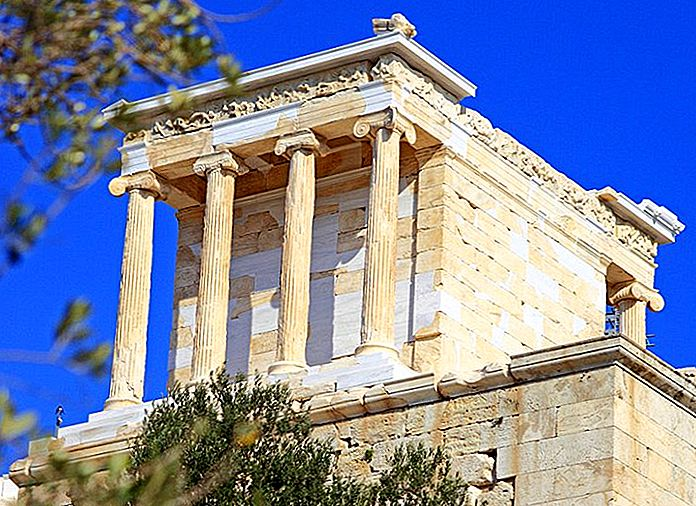
\includegraphics[width=1.0\linewidth]{02/nike_temploma}}
\end{wrapfigure}

\paragraph{Niké temploma}
A kisméretű templom a győzelem istennője, Niké számára épült, és arányai, harmóniája valóban nőiességet és győzelmet tükröznek. A kis templomot lépcsős alépítmény emeli meg. Alaprajzi elrendezését tekintve a kettős prosztülosz (diprosztülosz vagy amfiprosztülosz) típusába tartozik: a (csaknem négyzetes) téglalap alakú falait a két rövidebbik oldalon oszlopos előcsarnok egészíti ki - a bejáratok előtt mindkét oldalon négy-négy ión stílusú oszlop áll.

\begin{wrapfigure}{r}{0.35\textwidth}
	\tcbox[colback=darkgray!85!black,
	left=0mm,right=0mm,top=0mm,bottom=0mm,boxsep=1mm,toptitle=0.5mm,bottomtitle=0.5mm,
	title=\centering{Tholosz Delphoi-ban}]{
		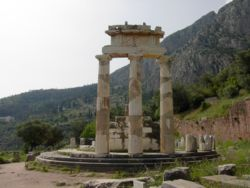
\includegraphics[width=1.0\linewidth]{02/delphoi_tholosz}}
\end{wrapfigure}


\paragraph{A Delphoi-i szent kerület}

Az összgörögség egyik legjelentősebb vallási központja Apollón delphoi-i jóshelye volt a Parnasszosz hegységen. A kultuszhely – mint a görög vallási helyek általában – a hegyoldalba épült, és több épületből állt. A hegy tetején volt Apollón temploma, ami az athéni Parthenónhoz hasonlóan dór stílusú peripterosz volt. A kincsesházak mellett egy kisméretű kör alaprajzú dór tholosz is épül itt. Apollón temploma alatt az uralkodók ajándékait őrző kisméretű
kincsesházak sorakoztak. Az Apollón templom melletti lejtőn épült fel a delphoi színház is, követve a színházak fent leírt kialakítását,

\subsubsection{Szobrászat}

\paragraph{Alapanyag}
Ettől a kortól kezdve a görög szobrok bronzból készülnek, gazdag aranyozással. Számos alkotás azonban márványból vagy más kőből maradt ránk. Ennek az az oka, hogy a területet meghódító rómaiak elszállították a görög szobrokat, részben hogy jelezzék a terület fölötti hatalmukat, részben pedig azért, hogy a bronzot beolvasztva abból fegyvereket gyártsanak. A görög szobrokról gyakran több példányban is készítettek másolatokat. Az alkotások nagy részét tehát csak római márvány másolatban ismerjük

\paragraph{Téma}
A sport, az Olümpiában tartott játékok igen fontos szerepet játszottak az ókori görög kultúrában. Eredetükben vallásos vonatkozásúak voltak, hiszen a játékok célja az volt, hogy az emberek megtudják, hogy ki az, akit az istenek a legyőzhetetlenség tulajdonságával ajándékoztak meg. A sportroló tehát egyben a görög társadalom hőse volt. A klasszikus korban a játékokat praktikus céllal is tartották, a katonáskodással függtek össze, hiszen a jó testfelépítésre szükség volt a háborúkban. A hazaszeretet, a szülőváros védelme pedig az egyik legfőbb férfierények közé tartozott. A sportos-katonás-hősies fiatal férfi így a társadalom mintaképévé vált.

\paragraph{Stílus}
A stílusban egyszerre két cél érvényesül: realitás – az archaikus kori kúroszokhoz képest élethűbb, plasztikusabb testfelépítés, izomzat, testtartás; idealizálás és tipizálás – minden szobor a kor ideális férfi-típusát igyekszik megfogalmazni.

\paragraph{Korszakok jellemzői}

	\subparagraph{Korai klasszikus szobrászat - Szigorú stílus}
	A stílus még őrzi az Archaikus kor kötött, merev ábrázolásmódjának hagyományait, de már érzékelhető benne a mozgás, a test, az arc valósághű bemutatása iránti igény – ötvöződik az archaikus kor és az érett klasszikus kor stílusa.
	
	Az arcokról eltűnik az archaikus mosoly, a tekintetek komorak, szigorúak – ezért kapja a korszak a szigorú stílus elnevezést.
	
	\begin{wrapfigure}{r}{0.2\textwidth}
		\tcbox[colback=darkgray!85!black,
		left=0mm,right=0mm,top=0mm,bottom=0mm,boxsep=1mm,toptitle=0.5mm,bottomtitle=0.5mm,
		title=\centering{Delphoi-i kocsihajtó szobra}]{
			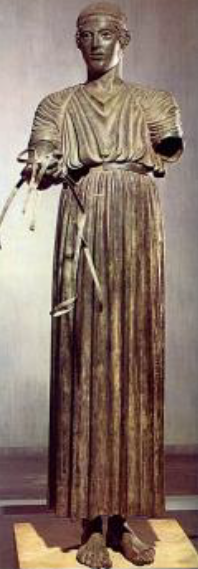
\includegraphics[width=1.0\linewidth]{02/kocsihajto_szobor}}
	\end{wrapfigure}
	
	\subparagraph{Szigorú stílusú szobor: kocsihajtó szobra (példa)}
	Egy győztes sportrolót látunk itt, akiben a nép az istenek kiválasztottját látta, ezért számára szobrot állíttatott.
	
	A stilizált, szinte csak a fej felületébe karcolt haj, a szimmetrikus szemöldök még őrzi az Archaikus kor tradícióit, a szem, a száj és a széles áll megoldása viszont már valósághű, már-már portrészerű vonás, nem beszélve a színes berakott szemekről és a szobornak életteli tekintetet kölcsönző szempillákról. A figura felépítéséből eltűnik a frontalitás, a fej, a törzs kimozdul a tengelyből, a testtartás mégis még mindig merev. Az alak egyszerű mozdulatot tesz – valaha a kantárokat tartotta.
	
	Az alakot ruha takarja, a drapéria még a kóré-szobrok sűrű, monoton, egyforma redőinek hatását tükrözi, csak a derék övénél érzékelhető rajta variáció.
	
	\subparagraph{Érett klasszikus szobrászat - Periklész kora (Kr. e. 450-430)}
	Az államférfi vezetése alatt politikai és társadalmi egyensúly jellemzi Athén életét, virágzik a demokrácia. Periklész – aki az egyik legfőbb megrendelőként lép fel – a fáradtságtól, szenvedéstől, öregségtől, betegségtől mentes virágzó athéni jólétben élő embert kívánja bemutattatni a művészet által is. A művészet célja az lesz, hogy az athéni ifjak elé az erős, sportos, katonaként hősies, ideális athéni polgárt állítsa: a szobrászat fő témája így továbbra is az ember, az izmos, harmonikus férfitest lesz.
	
	\begin{itemize}
		\item \textbf{Polükleitosz}: kidolgozza a „tökéletes emberi arányok” elméletét, írását ki is adják. Az ő nevéhez fűződik a kontraposzt szerkesztési elvének feltalálása, tudatos alkalmazása.
		\begin{compactitem}
			\item \textbf{Kontraposzt tartás}: A figura az egyik lábára támaszkodik, arra helyezik a testsúlyt, míg a másik lábát lazán, behajlítva tartja. Az kifejezés az olasz „contrapposto” szóból származik, ami ellentétet jelent, és a két láb ellentétes tartására utal. A kontraposzt tartás jóval életszerűbb, mint a frontális beállítás volt, kiegyensúlyozottságot, nyugalmat tükröz, ugyanakkor a behajlított láb bármikor mozgásba jöhet, ezért a tartásban a tettrekészség is megnyilvánul. Lazaságot, magabiztosságot, büszkeséget is érzékeltet.
			
			\item \textbf{Dárdavivő}: A szobor címe szerint témája egy dárdáját vivő férfit látunk, aki lehet egy katona, de lehet egy sportroló is. A témában is megjelenik a klasszikus kor célja – bemutatni azt az ideális férfitípust, aki egyszerre sportos, katonás, hősies. A szobor testfelépítése plasztikus, az izmok élesen elkülönülnek egymástól, minden izom külön ki van faragva, minden kis izom önálló plasztikai tömböt alkot, az erőt jeleníti meg. Arca nyugodt, érzelmektől mentes, fiatal, idealisztikus – ránctalan, szimmetrikus, kissé nyitott dús száj, görögös arcél (= a homlok és az orr találkozásánál nincsen mélyedés, orrnyereg).
			
			\item \textbf{Győzelmi szalagos ifjú}: Testfelépítésében, testtartásában megegyezik a Dárdavivővel. A szobor egy olyan sportroló ifjút ábrázol, aki a győzelem után szalagját köti a fejére.
			
		\end{compactitem}
	
		\item \textbf{Mürón : Diszkoszvető}
		\begin{compactitem}
			\item A szobor a görög művészet talán legismertebb alkotása, ugyanis kivételt, különlegességet képvisel a klasszikus kori szobrászatban: ilyen bonyolult, csavart testtartással csak a hellenizmusban fogunk találkozni. A szobor bronz eredetije elveszett, római márvány-másolatokból ismerjük.
			
			\item Témája a korongot elhajítani készülő atléta.
			
			\item A szobor látszólag egy mozdulatsor egyetlen pillanatát, az atléta lendületvétele utáni nyugvópontot ábrázolja, amikor a sportoló karja éppen leghátrébb van a korong elhajítása előtt. Ez a pillanat azonban fényképfelvételek tanúsága szerint nem létezik a valóságban, ráadásul a diszkoszvető a valóságban vízszintesen tartja a korongot, ha úgy tartaná, ahogy Mürón figurája, legfeljebb csak magasra, semmiképp sem messzire hajíthatná el.
			
			\item Mürón tehát nem szigorú valósághűségre törekedett, hanem a diszkoszvető mozgásáról alkotott tudást sűrítette egyetlen kompozícióba.
		\end{compactitem}
	
		\item \textbf{Pheidiász: Athéné Partenosz szobra}
		\begin{compactitem}
			\item A Parthenon cellája előtt hatalmas méretű bronzszobrot állít Pheidiász. Az eredeti alkotás 17 m magas volt, fából készült, amit drága anyagokkal borítottak: arannyal, elefántcsonttal, színes drágakövekkel vonták be. A szobor elveszett, csak római kori, nem túl hiteles márvány-másolatát ismerjük.
			
			\item Athéné figuráján a méltóságteljességen van a hangsúly: kontraposztban áll, ruhájának esése jól láttatja a testtartást. Nem a bölcsesség istennőjeként jelenik meg (olyankor baglyot tart a kezében), hanem Athén város védőisteneként: ezért attribútumai a győztes harcos jelképei: sisak, pajzs (mint a legtisztességesebb, védekezésre szolgáló fegyverek), és a győzelmet szimbolizáló Niké kis szobra, amit a kezében tart.
		\end{compactitem}
	\end{itemize}
	
	\begin{figure}[H]
		\centering
		\begin{minipage}{0.3\textwidth}
			\begin{tcolorbox}[enhanced,colframe=gray!50!white,
				colbacktitle=white!15!white,
				coltitle=gray!50!black,
				borderline={0.5mm}{0mm}{gray!15!white},
				borderline={0.5mm}{0mm}{gray!50!white,dashed},
				attach boxed title to top center={yshift=-2mm},
				boxed title style={boxrule=0.4pt},
				title=Dárdavivő]{
					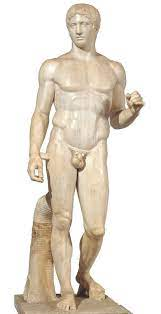
\includegraphics[width=1.0\linewidth]{02/dardavivo}}
			\end{tcolorbox}
		\end{minipage}
		\hfill
		\begin{minipage}{0.33\textwidth}
			\begin{tcolorbox}[enhanced,colframe=gray!50!white,
				colbacktitle=white!15!white,
				coltitle=gray!50!black,
				borderline={0.5mm}{0mm}{gray!15!white},
				borderline={0.5mm}{0mm}{gray!50!white,dashed},
				attach boxed title to top center={yshift=-2mm},
				boxed title style={boxrule=0.4pt},
				title=Diszkoszvető]{
				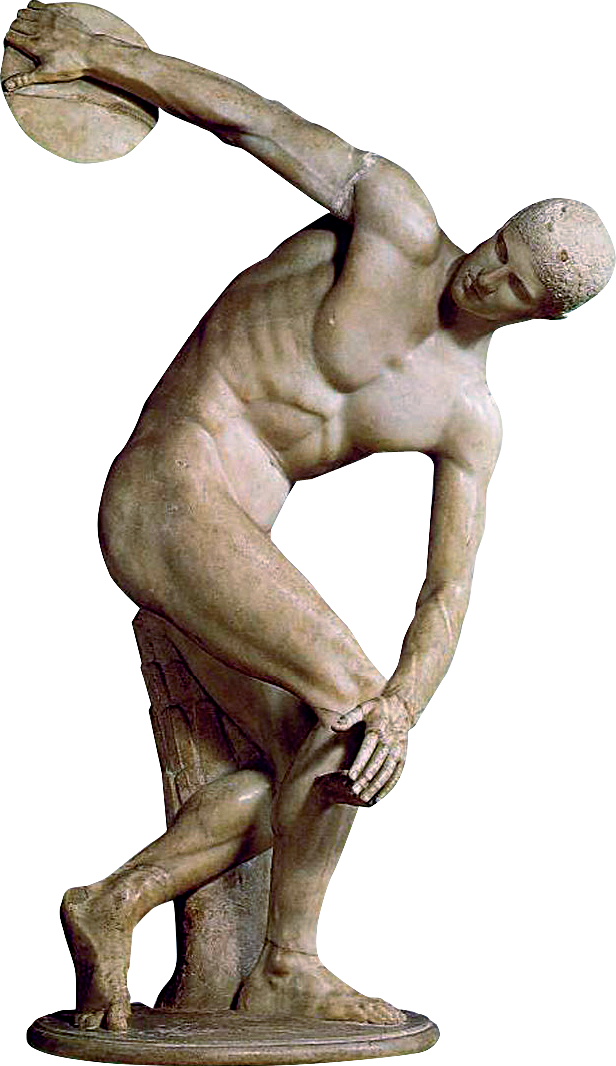
\includegraphics[width=1.0\linewidth]{02/diszkoszveto}}
			\end{tcolorbox}
		\end{minipage}
		\hfill
		\begin{minipage}{0.27\textwidth}
			\begin{tcolorbox}[enhanced,colframe=gray!50!white,
				colbacktitle=white!15!white,
				coltitle=gray!50!black,
				borderline={0.5mm}{0mm}{gray!15!white},
				borderline={0.5mm}{0mm}{gray!50!white,dashed},
				attach boxed title to top center={yshift=-2mm},
				boxed title style={boxrule=0.4pt},
				title=Athéné Partenosz]{
					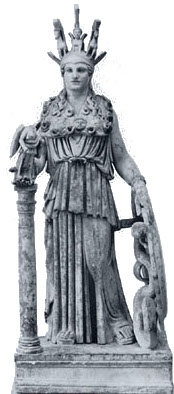
\includegraphics[width=1.0\linewidth]{02/athene}}
			\end{tcolorbox}
		\end{minipage}
		\captionsetup{labelformat=empty}
		\caption{}
	\end{figure}
	
	\subparagraph{Késő-klasszikus kori szobrászat}
	A peloponésszoszi háborúban Athén alulmarad Spártával szemben, majd a IV. században a katonáskodás teljesen megszűnik a polgárság számára, Athén katonái ettől az időtől kezdve zsoldosok lesznek. A katonáskodás és a sport ideje leágazóban van, megszűnik a hősies atléták kultusza. A szobrászatban sem a példakép-állítás lesz a cél, a művészet nem tanít többet, és nem állít ideált az athéni ifjak elé. A művészet célja egyre inkább a \textbf{gyönyörködtetés és az érzelmek megragadása} lesz.
	
	A hangsúly elterelődik az izmos férfitestről, összefogottabb, kevésbé részletesen bemutatott testfelépítés lesz jellemző. Az ábrázolásban a mitológiai történetek bensőséges érzelemvilágának láttatása kerül az előtérbe.
	
	\begin{itemize}
		\item \textbf{Praxitelész: Hermész a kis Dionüszosszal}
		\begin{compactitem}
			\item A késő-klasszikus korban a hangsúly a harmonikus férfitest helyett a mitológiai történet bensőséges ábrázolására kerül: férfi és gyermek kapcsolatát mutatja be a szobor.
			
			\item Téma: Zeusz Hermészre bízza újszülött fiát, hogy Héra a haragja elől a nimfákhoz vigye a gyermeket. Az úton megpihennek, és Hermész szőlővel eteti meg a leendő boristen-gyermeket. (A szőlő a szoborról mára letört.)
			
			\item Stílus: Nem aprólékosan felépített izomzatot, hanem finoman, harmonikusan összefogott férfitestet látunk. A késő-klasszikus szobrászatnak nem célja, hogy minden izmot külön megfaragva bemutasson, nem célja, hogy az erőt, a férfiasságot tükrözze.
		\end{compactitem}
	
		\item \textbf{Praxitelész: Knidoszi Aphrodité} Az első ruhátlan nőalak. Praxitelész szakít a ruhás nőalakok ábrázolásával, és ezzel megteremti a mezítelen görög Afrodité szobrok típusát, ami azt a témát ábrázolja, amikor Afrodité a szépség és szerelem istennője fürdőzik.		
	\end{itemize}

	\begin{figure}[H]
		\centering
		\hfill
		\begin{minipage}{0.35\textwidth}
			\begin{tcolorbox}[enhanced,colframe=gray!50!white,
				colbacktitle=white!15!white,
				coltitle=gray!50!black,
				borderline={0.5mm}{0mm}{gray!15!white},
				borderline={0.5mm}{0mm}{gray!50!white,dashed},
				attach boxed title to top center={yshift=-2mm},
				boxed title style={boxrule=0.4pt},
				title=Hermész Dionüszosszal]{
					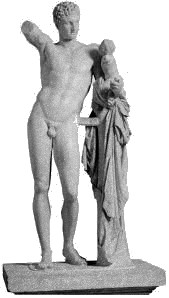
\includegraphics[width=1.0\linewidth]{02/hermesz_dionuszosszal}}
			\end{tcolorbox}
		\end{minipage}
		\hfill
		\begin{minipage}{0.27\textwidth}
			\begin{tcolorbox}[enhanced,colframe=gray!50!white,
				colbacktitle=white!15!white,
				coltitle=gray!50!black,
				borderline={0.5mm}{0mm}{gray!15!white},
				borderline={0.5mm}{0mm}{gray!50!white,dashed},
				attach boxed title to top center={yshift=-2mm},
				boxed title style={boxrule=0.4pt},
				title=Knidoszi Aphrodité]{
					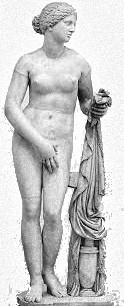
\includegraphics[width=1.0\linewidth]{02/knidoszi_afrodite}}
			\end{tcolorbox}
		\end{minipage}
		\hfill
		\captionsetup{labelformat=empty}
		\caption{}
	\end{figure}
	

\subsubsection*{Vázafestészet}

\begin{wrapfigure}{r}{0.4\textwidth}
	\begin{tcolorbox}[enhanced,colframe=gray!50!white,
		colbacktitle=white!15!white,
		coltitle=gray!50!black,
		borderline={0.5mm}{0mm}{gray!15!white},
		borderline={0.5mm}{0mm}{gray!50!white,dashed},
		attach boxed title to top center={yshift=-2mm},
		boxed title style={boxrule=0.4pt},
		title=Vörös alakos váza]{
			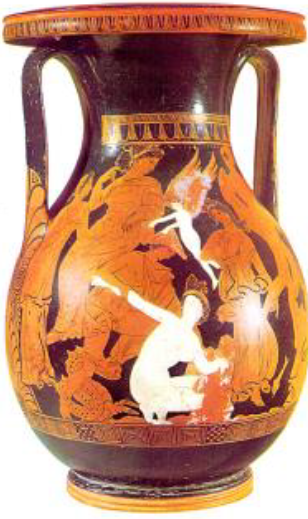
\includegraphics[width=1.0\linewidth]{02/voros_alakos_vaza}
			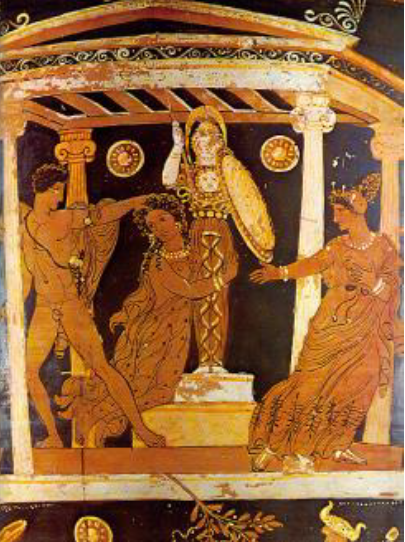
\includegraphics[width=1.0\linewidth]{02/voros_alakos_vaza_resze}
		}			
	\end{tcolorbox}
\end{wrapfigure}

Kialakul a \textbf{vörösalakos stílus}.

A terrakotta felületen \textbf{a figurát hagyják máz nélkül, ezért az vörös marad}, és a többi részt festik be fekete mázzal, \textbf{a figura tehát úgy alakul ki, hogy körbe van festve}.

A korábban (archaikus korban) kialakult fekete alakos vázáknál a fekete mázas rész volt a figura, és a részleteket ebbe a fekete mázba bekarcolt vonalakkal dolgozták ki.

A vörös alakos vázáknál a részletek bemutatását a festetlenül hagyott vörös felületen hajszálvékony fekete mázzal húzott ecsetvonásokkal érik el.

Ez a technikai megoldás nehezebb, mint a korábbi, hiszen a figurát kell körberajzolni, de mégis \textbf{népszerűbbé válik}, mert az \textbf{ecsetvonásokkal aprólékosabb}, könnyedebb, lendületes vonalrajzra nyílt lehetőség.

A kompozíciók \textbf{kevés alakosak}, a \textbf{figurák nagyobb méretűek}, mint korábban – az egész edényt betöltik.

Teljes mértékben \textbf{megszűnik a legnagyobb felületek törvénye}: a figurák profilból, szemből és rövidülésben egyaránt ábrázoltak, félprofilra, háromnegyedprofilra is találunk példát. A térben reális egymás-mögöttiség látszik.Az arcok a korábbiaknál valósághűbbek, érzelmek nyilvánulnak meg rajtuk.

A leggyakrabban ábrázolt téma továbbra is a mitológia, de itt a nem mítosz elmesélése a cél, hanem a \textbf{mitológiai jelenet emberibb, bensőséges pillanataira koncentráló bemutatása}.

\clearpage

\subsection*{A hellenizmus kora}

\paragraph{Történelem}
A hellenizmus kora Kr.e. 333-tól (Nagy Sándor fellépésétől) Kr.e. 30-ig (az actiumi csatáig, amikor Kleopártrát legyőzik a rómaiak, majd meghódítják a hellén világ területeit) tartott.

A makedón uralkodó, Philipposz a Kr.e. IV.sz. közepén terjeszkedni kezd a Peloponésszoszi félszigeten. A perzsák elleni összefogás ürügyén szövetséget köt a görög városállamokkal, egyesíti Makedóniát és Görögországot, létrehozza a görög hegemóniát, aminek ő lesz a vezetője.

Philipposz halála után fia, Alexandrosz válik a görögség vezetőjévé, aki mindössze húsz éves ekkor. Alexandrosz hatalmas hadsereget hoz létre, és Kr.e. 333-ban elindul kelet felé, hogy a perzsáktól visszahódítsa a görög területeket. Ám nem csak a Peloponésszoszi félszigetet és Kis-Ázsia partvidékét tisztítja meg a perzsáktól, hanem további területeket hódít meg: Egyiptomot, Szíriát, Mezopotámiát és a mai Irán és Afganisztán területét, az egész egykori Perzsiát. (India nyugati határáig jut el.) Alexandroszt nagy hódításai miatt a történelemben Nagy Sándorként szerepel.

A meghódított vidékeken Nagy Sándor új városokat alapít, amiket gyakran magáról neveztet el. Ezeknek leghíresebb példája az Egyiptom északi partvidékén alapított Alexandria.

Nagy Sándor halála után hadvezérei három részre osztják fel a birodalmat. Mindhárom terület hatalmának a rómaiak hódításai vetnek véget a Kr.e. I. században.

\paragraph{Elnevezés}
A „hellén” szó görögöt jelent, erről kapja a nevét a korszak, azért, mert a Nagy Sándor által meghódított birodalom utódállamaiban évszázadokon át a görög kultúra és eszmevilág hatása érvényesül.

\paragraph{Kultúra}
Mivel Nagy Sándor görögnek tartja magát, mindenhol a görög nyelv lesz a hivatalos, így a görög kultúra óriási földrajzi területen fejti ki hatását. A megrendelők egyrészt az uralkodók, másrészt a magánszféra lesznek. A hellenizmus szellemiségére a sokféleség jellemző.

\subsubsection{Építészet: A hellenisztikus város}

A korábbi görög korok építészete elsősorban a templomépítészetre koncentrált. A hellenizmusban a városalapítások miatt az építészetben a várostervezés és a középületek válnak a legfontosabbá.

\vspace{0.5cm}

\tcbox[colback=darkgray!85!black,
left=0mm,right=0mm,top=0mm,bottom=0mm,boxsep=1mm,toptitle=0.5mm,bottomtitle=0.5mm,
title=\centering{Egy hellenisztikus város rajza}]{
	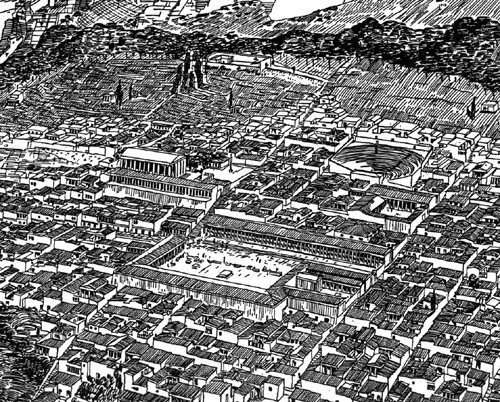
\includegraphics[width=1.0\linewidth]{02/hellenizmus_varos}}

\paragraph{Városépítés elve}
Hippodámoszi elvek = Hippodámosz görög építész volt, aki kidolgozta a hellén városok építésének módszerét. A módszer lényege, hogy a teljesen újonnan létesítendő várost előre megtervezik, négyszögletes városalaprajzot, szabályos utcahálózatot készítenek. A város egyes részeinek funkcióját előre meghatározzák aszerint, hogy az politikai, társadalmi, közigazgatási vagy vallási célokra alkalmasabb-e. Az egyik leghíresebb hellénisztikus város Pergamon.

\clearpage

\paragraph{Épülettípusok}

	\subparagraph{Agóra}
	A városban általában egy fő út húzódott végig. A központban ezt az utat kiszélesítve alakították ki \textbf{a város hosszúkás főterét, az agórát}. Az agóra a város kereskedelmi, közigazgatási, politikai életének központja volt. Oldalain a kereskedelemhez, a bíráskodáshoz és a törvényhozáshoz kapcsolódó épületek álltak.
	
	\subparagraph{Sztoa}
	Az agóra hosszanti oldalán álló sétacsarnok vagy \textbf{kereskedelmi oszlopos csarnok}. Az épület kezdetben a hátoldalán zárt volt, az agóra felé pedig oszlopcsarnokkal vagy oszlopos folyosóval nyitott. Hosszanti elrendezésű, általában kéthajós volt: egy belső oszlopsor osztotta két részre.
	
	\subparagraph{Buleutérion}
	A sztoa rövidebbik végén álló épület, a \textbf{görög vének tanácsának (a bulénak) tanácskozó, ülésező helye}, az antik görögség „parlamentje”.
	
	\subparagraph{Gümnaszion}
	Épületegyüttes, ami az ifjúság testi nevelését szolgálta.
	
	\subparagraph{Stadion}
	Az atlétikai versenyek színhelye volt. Hosszúkás alaprajzú, nyitott versenypálya, az egyik vége négyszögletesen, a másik lekerekítetten záródott.
	
	\subparagraph{Hippodron}
	Lóverseny és kocsihajtó verseny pálya. Szintén nyújtott téglalap alakú egyik végén lekerekítve.
	
	\subparagraph{Szelek tornya}
	Olyan kisméretű torony az agóra közelében, ami víziórával és napórával volt ellátva, és az idő mellett a széljárást is mutatta.
	
	\subparagraph{Lakóházak}
	A hellenizmus embere zsúfolt városokban, új típusú házban élt. A házak közvetlenül egymás mellé épültek, ezért a falakon nem voltak ablaknyílások. A ház egy téglalap alakú központi nyitott udvar köré épült fel. Az udvar négy oldalán az udvar felé nyitott, oszlopos folyosók voltak.
	
	Az udvar körül helyezkedtek el a lakóhelyiségek, amiknek nem volt ablakuk, a fény csak az udvar felé nyíló ajtókon keresztül szivárgott be.
	
	A leghíresebb hellenisztikus lakóházak Déloszban maradtak fenn.

\subsubsection{Szobrászat}

\begin{wrapfigure}{r}{0.32\textwidth}
	\tcbox[colback=darkgray!85!black,
	left=0mm,right=0mm,top=0mm,bottom=0mm,boxsep=1mm,toptitle=0.5mm,bottomtitle=0.5mm,
	title=\centering{Szamothrakéi Niké}]{
		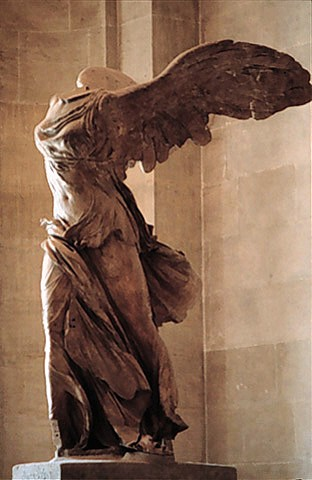
\includegraphics[width=1.0\linewidth]{02/szamothrakei_nike}}
	
	\begin{tcolorbox}[enhanced,colframe=gray!50!white,
		colbacktitle=white!15!white,
		coltitle=gray!50!black,
		borderline={0.5mm}{0mm}{gray!15!white},
		borderline={0.5mm}{0mm}{gray!50!white,dashed},
		attach boxed title to top center={yshift=-2mm},
		boxed title style={boxrule=0.4pt},
		title=Guggoló Aphrodité]{
			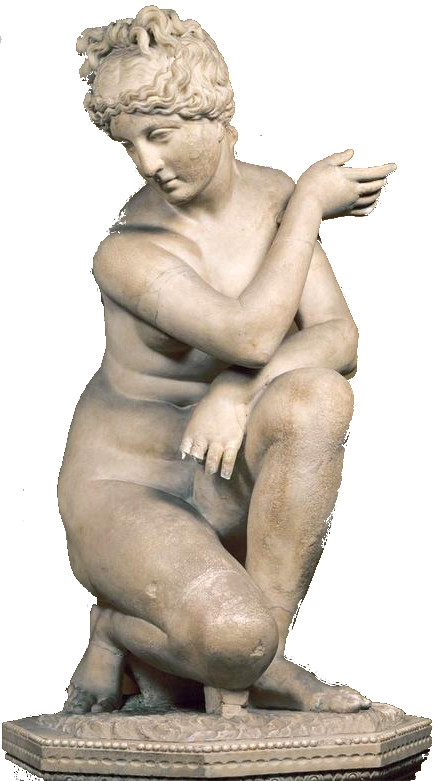
\includegraphics[width=1.0\linewidth]{02/guggolo_aphrodite}
		}			
	\end{tcolorbox}

	\tcbox[colback=darkgray!85!black,
	left=0mm,right=0mm,top=0mm,bottom=0mm,boxsep=1mm,toptitle=0.5mm,bottomtitle=0.5mm,
	title=\centering{Alvó Érosz}]{
		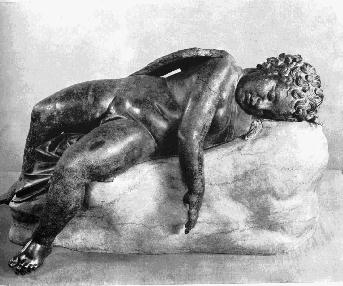
\includegraphics[width=1.0\linewidth]{02/alvo_erosz}}
\end{wrapfigure}

\paragraph{Rendeltetése}
Az alkotások nagy része magánmegrendelésre készül. Míg a klasszikus kori szobrászatban az állam tükrözni akarta, hogy polgára mily egészséges, szép, stb., addig a hellenizmus privát megrendelői a mindennapi valóságot kívánták láttatni. Míg a klasszikus korban a harmónia dominált, a hellenizmus szinte föllázad a már-már kánonná, kötelezővé vált harmónia ellen, és célja az, hogy az életet akár szép, akár csúnya oldaláról, de mindenképpen \textbf{reálisan, naturalisztikusan} mutassa be.

\paragraph{Új témák}

	\subparagraph{A görög mitológia alakjai, istenei emberi módon ábrázolva}
	
	Szamothrakéi Niké: A Győzelem istennője éppen egy hajó orrára száll le. Hátán még szétnyitva állnak szárnyai, testére, combjára rátapad a ruha, lábán a hátrafelé hullámzó drapéria tükrözi a lendületet, amivel érkezik. A női test korábban nem látott szépségű és reális megfogalmazásával állunk szemben.
	
	\subparagraph{A nő}
	
	 Guggoló Aphrodité: Mitológiai témaként (a fürdőző Afroditét ábrázolja, amikor magára önti a vizet) jelenik meg a női akt, de megfogalmazásmódja reális és érzéki.
	
	\subparagraph{A gyermek}
	
	Alvó Érosz: A gyermek arányait, testfelépítését, a puha, elernyedt testrészeket, a gyermeki természetet, az alvás pillanatát mind reálisan, és érzékletesen ábrázolta az alkotó.
	
\clearpage	
	
	\subparagraph{Jellem- és lélek-ábrázolás}
	
	Libát fojtogató kisfiú: A gyermeki természet igen érdekes bemutatása, amikor a gyermek pontosan tudja, hogy ki az a lény, akinél ő feljebb való, és megtalálva méltó ellenfelét a világban, tudatlanságával kifejezi erejét a védtelen állat felett. A gyermek arcán látszik a küzdelem, karjai megfeszülnek, a liba az életéért küzd.
	
	\subparagraph{A táncos, maga a mozgás}
	
	Táncosnő: A táncosnő-ábrázolások elterjedéséhez minden bizonnyal hozzájárult a keleti táncok megjelenése, ahol a nőiesség, a kidomborodó női formák és az eltakaró leplek kettőssége kelti a feszültséget. A táncosnő-szobrok a forgó mozgást ragadják meg, gyakori jellemzőjük a kidugott könyökre ráfeszülő drapéria motívuma.
	
	\subparagraph{A rút, a csúnya, a torz, a groteszk, az élet elrettentő oldalai}
	
	A klasszikus korban kizárólagosan ideálisan ábrázolt ember alakjaival ellentétben a hellenisztikus szobor kíméletlenül mutatja be az emberi fizikum torzulásait.
	
	Bokszolófej: szinte kigúnyolja ez a szoborfej a klasszikus kori szobrászat sportroló ábrázolásainak naiv idealizmusát, és azzal szemben a sportágat valós oldaláról közelíti meg, naturalisztikusan ábrázolja a durva sport fizikális következményeit.
	
	\begin{figure}[H]
		\begin{minipage}{0.3\textwidth}
			\tcbox[colback=darkgray!85!black,
			left=0mm,right=0mm,top=0mm,bottom=0mm,boxsep=1mm,toptitle=0.5mm,bottomtitle=0.5mm,
			title=\centering{Libát folytogató kisfiú}]{
				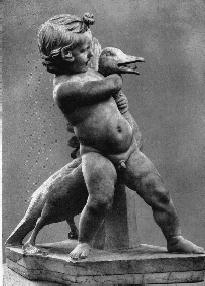
\includegraphics[width=1.0\linewidth]{02/libat_fojtogato}}
		\end{minipage}
		\hfill
		\begin{minipage}{0.33\textwidth}
			\begin{tcolorbox}[enhanced,colframe=gray!50!white,
				colbacktitle=white!15!white,
				coltitle=gray!50!black,
				borderline={0.5mm}{0mm}{gray!15!white},
				borderline={0.5mm}{0mm}{gray!50!white,dashed},
				attach boxed title to top center={yshift=-2mm},
				boxed title style={boxrule=0.4pt},
				title=Táncosnő]{
					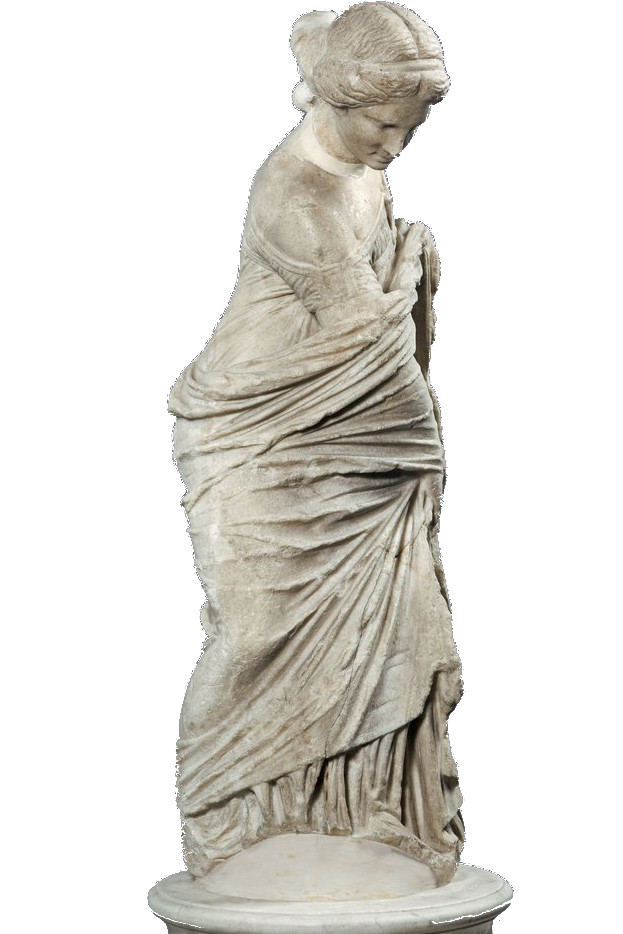
\includegraphics[width=1.0\linewidth]{02/tancosno}
				}			
			\end{tcolorbox}
		\end{minipage}
		\hfill
		\begin{minipage}{0.3\textwidth}
			\tcbox[colback=darkgray!85!black,
			left=0mm,right=0mm,top=0mm,bottom=0mm,boxsep=1mm,toptitle=0.5mm,bottomtitle=0.5mm,
			title=\centering{Bokszolófej}]{
				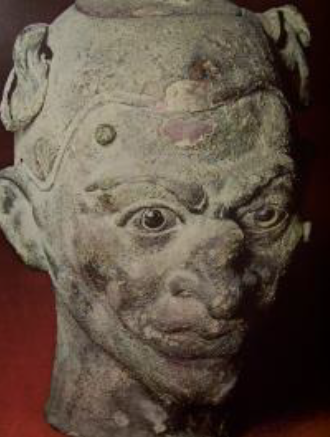
\includegraphics[width=1.0\linewidth]{02/bokszolofej}}
		\end{minipage}	
	\end{figure}

	\subparagraph{A szenvedés, a betegség}
	
	Részeg nő: Egyetlen szerelmeként és éltetőjeként szorítja magához a boros kancsót a nő, elalélt arcát az alkoholizmus ráncossá, öreggé, testét, mellkasát szikkadttá, ruházatát igénytelenné tette.
	
	Vödröt cipelő nő: A szegényes ruházatú asszony majd megszakad a vödör súlyától, melléről elcsúszott a ruha, arcán szenvedés és reménytelenség tükröződik, teste megfáradt.
	
	\begin{wrapfigure}{r}{0.45\textwidth}
		\begin{minipage}{0.22\textwidth}
			\tcbox[colback=darkgray!85!black,
			left=0mm,right=0mm,top=0mm,bottom=0mm,boxsep=1mm,toptitle=0.5mm,bottomtitle=0.5mm,
			title=\centering{Részeg nő}]{
				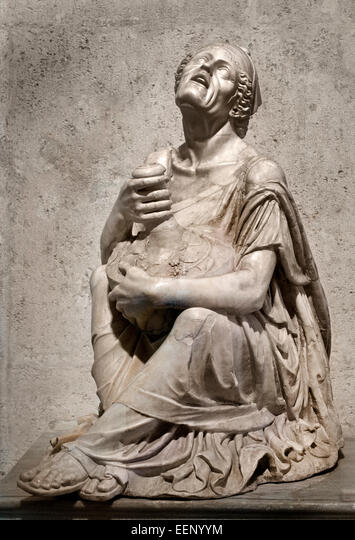
\includegraphics[width=1.0\linewidth]{02/reszeg_no}}
		\end{minipage}
		\hfill
		\begin{minipage}{0.2\textwidth}
			\tcbox[colback=darkgray!85!black,
			left=0mm,right=0mm,top=0mm,bottom=0mm,boxsep=1mm,toptitle=0.5mm,bottomtitle=0.5mm,
			title=\centering{Tövishúzó}]{
				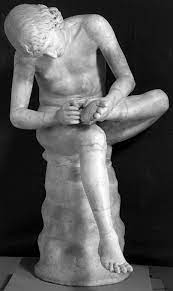
\includegraphics[width=1.0\linewidth]{02/tovishuzo}}
		\end{minipage}	
	
		\vspace{0.5cm}
	
		\begin{minipage}{0.45\textwidth}
			\begin{tcolorbox}[enhanced,colframe=gray!50!white,
				colbacktitle=white!15!white,
				coltitle=gray!50!black,
				borderline={0.5mm}{0mm}{gray!15!white},
				borderline={0.5mm}{0mm}{gray!50!white,dashed},
				attach boxed title to top center={yshift=-2mm},
				boxed title style={boxrule=0.4pt},
				title=Laokoón-csoport]{
					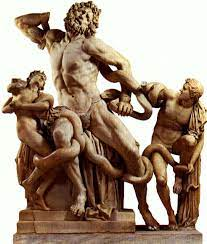
\includegraphics[width=1.0\linewidth]{02/laokoon}
				}			
			\end{tcolorbox}
		\end{minipage}	
	\end{wrapfigure}
	
	\subparagraph{Hétköznapi cselekmények}
	
	Tövishúzó: Korábban nem látott életszerűséggel jeleníti meg az alkotó az élet egy rendkívül profán pillanatát, amikor az ember lábába szálka megy. A fiatal, portrészerű vonásokat mutató, nagy orrú fiú, vézna teste, élethű testtartása a hellenizmus kíméletlen realizmusát, naturalizmusát mutatja.

\paragraph{Stílus}
	A stílusban is a sokszínűség érvényesül.
	
	Általában szabadon álló, minden oldalukkal érvényesülő, térben elhelyezett, sokalakos kompozíciók, körüljárható szobrok.
	
	Dinamikus, mozgalmas kompozíciók. A testtartások változatosak, élethűek, bonyolult, csavart testtartásokkal is találkozunk.
	
	A hellenizmus stílusában minden tekintetben a realizmus, sőt a kíméletlen naturalizmus kapja a fő szerepet.	
	
	A testfelépítés reálisan ábrázolt. Az arcok élethűek, változatos érzelmeket fejeznek ki, az érzelmek mellett az életkorok is változatosan és reálisan ábrázoltak; az arcokon a pszichológiai jellemzők is láthatók.
	
	A drapéria rendkívül változatosan jelenik meg, különböző minőségű anyagokat jelenít meg: vékony áttetsző anyagtól a vastagabb, súlyos anyagokig, általában követi a test formáját, azaz gyakran rátapad a testre. Így a ruha alatt látszik a test formája.

\cleardoublepage

\section{Az ókori görög kultúra festészetének hatása a római kori festészetre}

\tcbox[left=0mm,right=0mm,top=0mm,bottom=0mm,boxsep=0mm,
toptitle=0.5mm,bottomtitle=0.5mm,title=\centering{A tétel adatai}]{%	
\begin{tabular}{| p{0.25\textwidth} | p{0.7\textwidth} |}
	
	\hline
	Tétel teljes címe &
	Milyen módon, mértékben hatottak az ókori görög kultúra festészeti megoldásai tartalmi, formai, technikai szempontból a római kor festészetére? Milyen ókori mozaiktechnikákat ismer?
	\\ \hline
	
\end{tabular}}

\subsection*{A görög festészet}

Az ókori görög festészet fennmaradt alkotásai közül a festett vázák a legjelentősebbek, melyeket az A) részben már részleteztünk (geometrikus, orientalizáló, feketealakos és vörösalakos stílus).

 Falfestészetükről csak a római kori másolatok maradtak meg.

Az ókori Görögországban alakult ki a mozaik technika, de a római kultúra fejlesztette tovább.

\subsection*{Ókori mozaik technikák}

\paragraph{Szögmozaik (Mezopotámia)}
A mozaik első alkalmazásával a mezopotámiai művészetben találkozhatunk, amikor a nedves agyagba színes mázas homlokfelületű kúpokat (szögmozaik) nyomtak, így állítottak elő különböző, többnyire geometrikus mintájú díszítéseket. Ezek a leletek az uruki Vörös templomból kerültek elő, amelynek részletei a berlini Pergamon Múzeumban láthatók. Ezek a korai mozaikok valóban mozaikok ugyan, ami a raszterszerű megjelenésükből adódik, de agyagmozaikok, a kúpok homlokfelületét színes mázzal vonták be, és éppen ezért a felület megjelenése sokkal inkább a kerámiára emlékeztet, mint a megszokott értelemben vett mozaikra.

\begin{tcolorbox}[enhanced,colframe=gray!50!white,
	colbacktitle=white!15!white,
	coltitle=gray!50!black,
	borderline={0.5mm}{0mm}{gray!15!white},
	borderline={0.5mm}{0mm}{gray!50!white,dashed},
	attach boxed title to top center={yshift=-2mm},
	boxed title style={boxrule=0.4pt},
	title=A szögmozaik technika]{
		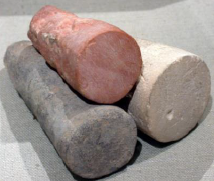
\includegraphics[width=0.31\linewidth]{02/szogmozaik_1}
		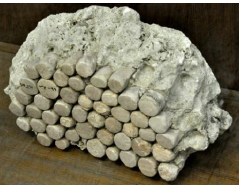
\includegraphics[width=0.35\linewidth]{02/szogmozaik_2}
		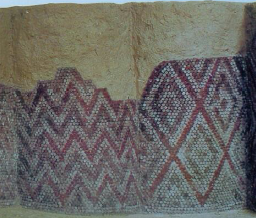
\includegraphics[width=0.31\linewidth]{02/szogmozaik_3}
	}
\end{tcolorbox}

\paragraph{Kavicsmozaik (Makedónia)}
A makedón fővárosban, Pellában is találtak mozaikokat. Az 1953-ban elkezdődött ásatások során \textbf{geometrikus mintázatú padlómozaikok} kerültek elő, \textbf{kavicsból kirakva}, az igazi szenzációt azonban a különböző jeleneteket (oroszlánon lovagló Dionüszosz, szarvas vadászat, oroszlánvadászat) ábrázoló mozaikok jelentették. Ezeket a mozaikokat sokszínű – pontosabban a klasszikus négyszín-festészet koloritját mutató – kavicsokból állították össze, de voltak részek (például a hajfürtök), amihez előre elkészített terrakottát használtak, a kontúrokat pedig ólomsávokkal rajzolták meg. A kavicsszemek sokkal kisebb méretűek voltak a korábbiaknál, így a közöttük lévő rések is vékonyabbak lettek. A mozaikok készítői nem törekedtek nagyobb térmélység kialakítására, csupán semleges háttérből előtűnő, reliefszerű alakokat akartak ábrázolni, ugyanakkor azonban érezhető a törekvés a „valóságos” képekké formálásra.

\tcbox[colback=darkgray!85!black,
left=0mm,right=0mm,top=0mm,bottom=0mm,boxsep=1mm,toptitle=0.5mm,bottomtitle=0.5mm,
title=\centering{Kavicsmozaik: oroszlánvadászat}]{
	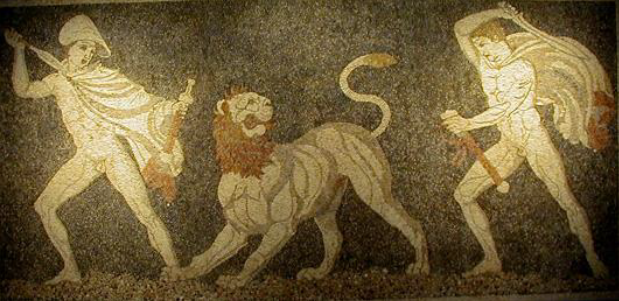
\includegraphics[width=1.0\linewidth]{02/kavicsmozaik}
}

\paragraph{Tesszera-mozaik (görög, római)}

\subparagraph{Kavicsok helyett szabályos, apró hasábok felhasználása}
A mozaiktechnika fejlődésében a következő – jelentős – lépésre az i. e. 3. században került sor. A mozaikok készítéséhez különböző színű kövekből, többé-kevésbé szabályos, apró hasábokat munkáltak ki. Az ilyen mozaiknak a neve „opus tessalatum” (kockás mű). A tesszera görög szó, a kis négyzetes hasábok neve.

\subparagraph{Speciális tesszara: négyszögletű, de nem négyzetes darabokból}
Amikor a hasábok nem négyzetesek, hanem négyszögletesek, a mozaik neve „opus sectile”. Alexandriából kerültek elő tesszera-mozaik töredékek. Az új mozaikok készítői közül néhányan kiváló művészekké váltak, akik nem ritkán szignatúrájukkal látták el a műveiket, így némelyiküket név szerint is ismerjük.

\subparagraph{A görög találmányt a rómaik vitték tovább}
A tesszera-mozaikot ugyan a görögök fejlesztették ki, mégis a római művészet tette naggyá; a rómaiak a középületeiket, fürdőépületeiket, lakóházaik padlóját díszítették mozaikkal. Ezek a korábbihoz képest megnövekedett épületbelsők gyakorlatilag megkívánták a padozat díszítését.

\tcbox[colback=darkgray!85!black,
left=0mm,right=0mm,top=0mm,bottom=0mm,boxsep=1mm,toptitle=0.5mm,bottomtitle=0.5mm,
title=\centering{Görög mozaikok}]{
	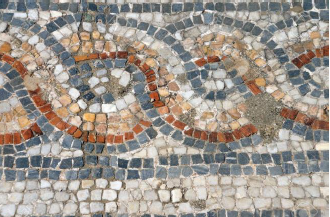
\includegraphics[width=0.49\linewidth]{02/gorog_mozaik_1}	
	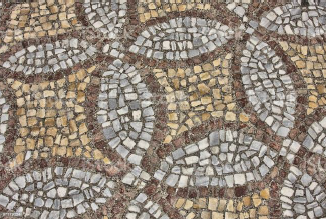
\includegraphics[width=0.5\linewidth]{02/gorog_mozaik_2}
}

\subparagraph{Készítésének menete}
Először kétszínű, majd a szőnyeghez hasonló, színes felületek voltak kedveltek. A díszítendő felület alá cementalapot készítettek, majd erre a teherviselő rétegre egy vékonyabb cement- vagy gipszréteg került. Ebbe nyomkodták bele a kis hasábocskákat. Nyilván olyan nagyságú felületet készítettek elő egyszerre, amit annak kötéséig el tudtak készíteni.

\subsection*{A római mozaik technika}

\paragraph{Eredete}
A mozaikokat a \textbf{görögök fejlesztették ki}, a görög mozaikok fekete-fehér (vagy inkább sötét és világos) kavicsokból kirakottak és geometrikus mintázatúak. Mégis a mozaik technika a római művészet által vált elterjedtté, ők fejlesztették tovább ezt a technikát. 

\paragraph{Témája}
A mozaikok, mint az egész ókori művészet, elbeszélő jellegűek, történetet vagy eseményt jelenítenek meg nagy természetességgel. 

\paragraph{A technika sokszínűsége}
A rómaiak fürdőépületeiket, középületeiket, lakóházaik padlóját díszítették mozaikokkal. A mozaikok falfestmények változataiként jöttek létre. A mozaikkészítés változatos és összetett mesterség volt: számos ágát (padló-, fal-, mennyezet-mozaik) és technikáját különböztették meg.

\subsubsection*{Híres római mozaikok}

Római kori mozaikok az egykori Római Birodalom egész területén találhatók. A római mozaikok tanulmányozásának két legfőbb helyszíne Pompeii és Herculaneum.

\paragraph{Nagy Sándor-mozaik}
A római mozaikok gyakran falfestmények másolataként jöttek létre. Az egyik legnevezetesebb római kori mozaikot, a Nagy Sándor-mozaikot, amely az isszoszi \textbf{csata jelenetét ábrázolja}, \textbf{Pompeiiben} tárták fel a "Faun házá"-ban, és a nápolyi Museo Archeologico Nazionale féltett kincse (a múzeumban függőleges helyzetben állították ki, de ez is \textbf{padlómozaik} volt). Mérete 2,71 x 5,12 méter. Keletkezését az i. e. 1. századra teszik. Mintája nagy valószínűséggel egy Philoxenosztól származó falfestmény volt, amelyet Rómában "sokszorosítottak".

\tcbox[colback=darkgray!85!black,
left=0mm,right=0mm,top=0mm,bottom=0mm,boxsep=1mm,toptitle=0.5mm,bottomtitle=0.5mm,
title=\centering{Nagy Sándor-mozaik}]{
	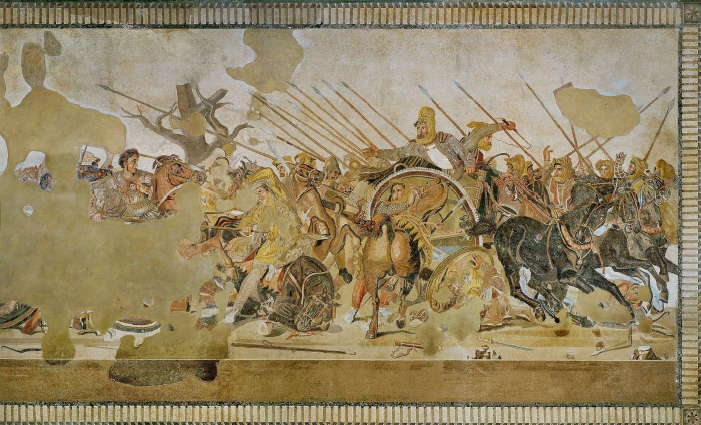
\includegraphics[width=1.0\linewidth]{02/nagy_sandor_mozaik}}

\paragraph{Cave canem (Őrizkedj a kutyától!) mozaikok}
Pompeiiben és Herculaneumban ezen kívül is számos mozaik került elő, például a Cave canem (Őrizkedj a kutyától!) mozaikok, amelyek a \textbf{lakóházak bejáratánál figyelmeztettek harapós kutyára}. Ezek annyira elterjedtek voltak \textbf{Pompei}iben, hogy még Petronius is megemlékezett róluk.

\begin{figure}[H]
	\begin{minipage}{0.47\textwidth}
	\tcbox[colback=darkgray!85!black,
	left=0mm,right=0mm,top=0mm,bottom=0mm,boxsep=1mm,toptitle=0.5mm,bottomtitle=0.5mm,
	title=\centering{Cave canem mozaik, Pompeii}]{
		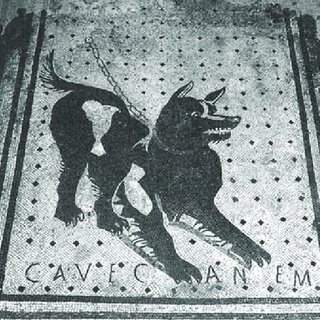
\includegraphics[width=1.0\linewidth]{02/cave_canem}}
	\end{minipage}
	\hfill
	\begin{minipage}{0.47\textwidth}
		\tcbox[colback=darkgray!85!black,
		left=0mm,right=0mm,top=0mm,bottom=0mm,boxsep=1mm,toptitle=0.5mm,bottomtitle=0.5mm,
		title=\centering{Platón a tanítványaival, Pompeii}]{
			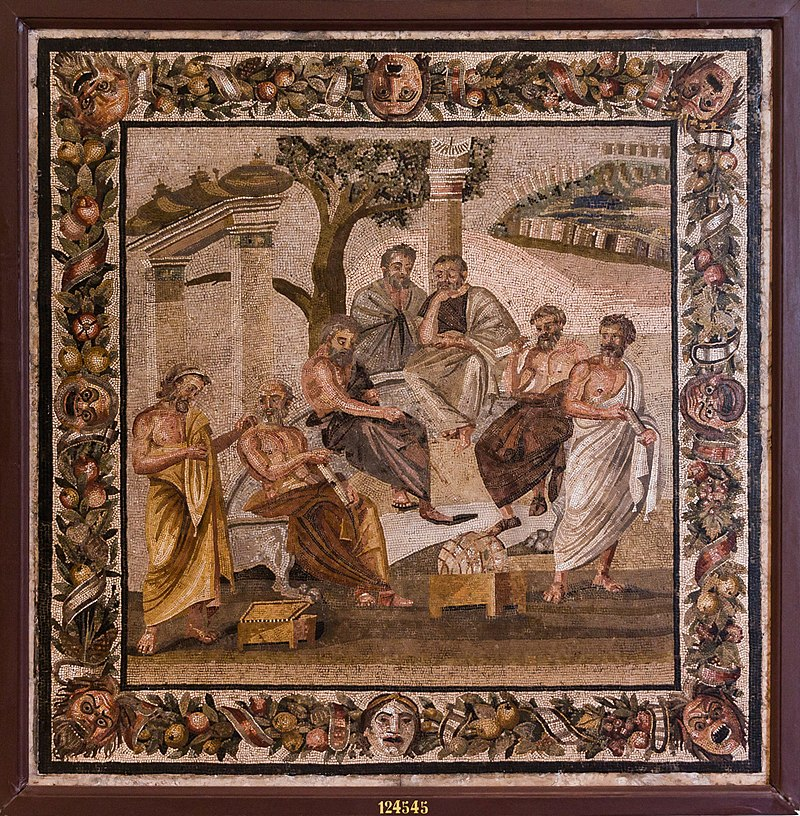
\includegraphics[width=1.0\linewidth]{02/platon}}
	\end{minipage}
\end{figure}

\subsection*{A mozaik technika}

A mozaik olyan művészeti technika és annak eredménye, amelynél kicsiny méretű színes üveg-, kő- vagy kavicsdarabokból állítják össze a képet vagy mintázatot (néha más anyagokat is használnak). A mozaikdarabokat cementtel, gipsszel rögzítik, esetleg a még nedves vakolatba nyomják bele. A mozaik szó a görög muszeion szóból eredeztetett latin opus musivum (múzsákhoz közelálló) kifejezésből származik. A művészeti ág múzsákkal való kapcsolatba hozása azt jelenti, hogy a mozaik igen megbecsült műfaj volt.

\vspace{2cm}

\section{Galéria}

\begin{figure}[H]
	\begin{minipage}{0.2\textwidth}
		\tcbox[colback=darkgray!85!black,
		left=0mm,right=0mm,top=0mm,bottom=0mm,boxsep=1mm,toptitle=0.5mm,bottomtitle=0.5mm,
		title=\centering{Archaikus kor, Dór oszloprend}]{
			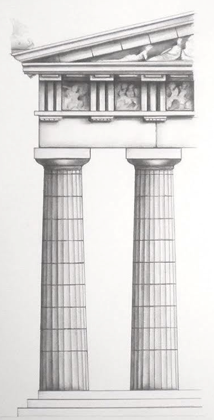
\includegraphics[width=1.0\linewidth]{02/01}}
	\end{minipage}
	\hfill
	\begin{minipage}{0.26\textwidth}
		\tcbox[colback=darkgray!85!black,
		left=0mm,right=0mm,top=0mm,bottom=0mm,boxsep=1mm,toptitle=0.5mm,bottomtitle=0.5mm,
		title=\centering{Archaikus kor, Ion oszloprend}]{
			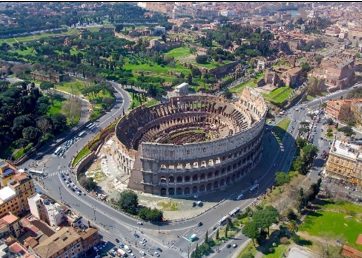
\includegraphics[width=1.0\linewidth]{02/02}}
	\end{minipage}
	\hfill
	\begin{minipage}{0.16\textwidth}
		\tcbox[colback=darkgray!85!black,
		left=0mm,right=0mm,top=0mm,bottom=0mm,boxsep=1mm,toptitle=0.5mm,bottomtitle=0.5mm,
		title=\centering{Klasszikus kor, Korintoszi oszloprend}]{
			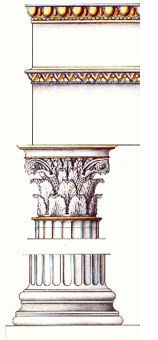
\includegraphics[width=1.0\linewidth]{02/03}}
	\end{minipage}
	\hfill
		\begin{minipage}{0.24\textwidth}
		\tcbox[colback=darkgray!85!black,
		left=0mm,right=0mm,top=0mm,bottom=0mm,boxsep=1mm,toptitle=0.5mm,bottomtitle=0.5mm,
		title=\centering{Klasszikus kor, feketealakos váza}]{
			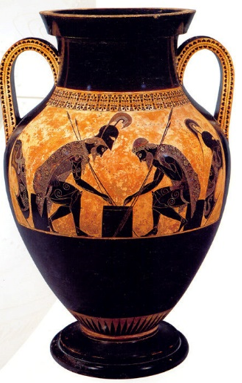
\includegraphics[width=1.0\linewidth]{02/07}}
	\end{minipage}
\end{figure}

\begin{figure}[H]
	\centering
	\begin{minipage}{0.34\textwidth}
		\tcbox[colback=darkgray!85!black,
		left=0mm,right=0mm,top=0mm,bottom=0mm,boxsep=1mm,toptitle=0.5mm,bottomtitle=0.5mm,
		title=\centering{Klasszikus kor, athéni Parthenon}]{
			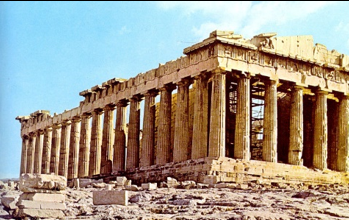
\includegraphics[width=1.0\linewidth]{02/04}}
	\end{minipage}
	\hfill
	\begin{minipage}{0.39\textwidth}
		\tcbox[colback=darkgray!85!black,
		left=0mm,right=0mm,top=0mm,bottom=0mm,boxsep=1mm,toptitle=0.5mm,bottomtitle=0.5mm,
		title=\centering{Parthenon alaprajza}]{
			\includegraphics[width=1.0\linewidth]{02/05}}
	\end{minipage}
	\hfill
	\begin{minipage}{0.22\textwidth}
		\tcbox[colback=darkgray!85!black,
		left=0mm,right=0mm,top=0mm,bottom=0mm,boxsep=1mm,toptitle=0.5mm,bottomtitle=0.5mm,
		title=\centering{Klasszikus kor, Niké templom}]{
			\includegraphics[width=1.0\linewidth]{02/06}}
	\end{minipage}

	\begin{minipage}{0.17\textwidth}
		\tcbox[colback=darkgray!85!black,
		left=0mm,right=0mm,top=0mm,bottom=0mm,boxsep=1mm,toptitle=0.5mm,bottomtitle=0.5mm,
		title=\centering{Archaikus kor, kúrosz}]{
			\includegraphics[width=1.0\linewidth]{02/08}}
	\end{minipage}
	\hfill
	\begin{minipage}{0.24\textwidth}
		\tcbox[colback=darkgray!85!black,
		left=0mm,right=0mm,top=0mm,bottom=0mm,boxsep=1mm,toptitle=0.5mm,bottomtitle=0.5mm,
		title=\centering{Klasszikus kor, Pheidiasz: Athéné Parthenon}]{
			\includegraphics[width=1.0\linewidth]{02/09}}
	\end{minipage}
	\hfill
	\begin{minipage}{0.17\textwidth}
		\tcbox[colback=darkgray!85!black,
		left=0mm,right=0mm,top=0mm,bottom=0mm,boxsep=1mm,toptitle=0.5mm,bottomtitle=0.5mm,
		title=\centering{Klasszikus kor, Polükleitosz: Dárdavivő}]{
			\includegraphics[width=1.0\linewidth]{02/10}}
	\end{minipage}
	\hfill
	\begin{minipage}{0.26\textwidth}
		\tcbox[colback=darkgray!85!black,
		left=0mm,right=0mm,top=0mm,bottom=0mm,boxsep=1mm,toptitle=0.5mm,bottomtitle=0.5mm,
		title=\centering{Klasszikus kor, Mürön: Diszkoszvető}]{
			\includegraphics[width=1.0\linewidth]{02/11}}
	\end{minipage}

	\begin{minipage}{0.4\textwidth}
		\tcbox[colback=darkgray!85!black,
		left=0mm,right=0mm,top=0mm,bottom=0mm,boxsep=1mm,toptitle=0.5mm,bottomtitle=0.5mm,
		title=\centering{Hellenizmus, Szamothrakéi Niké}]{
			\includegraphics[width=1.0\linewidth]{02/12}}
	\end{minipage}
	\hfill
	\begin{minipage}{0.57\textwidth}
		\tcbox[colback=darkgray!85!black,
		left=0mm,right=0mm,top=0mm,bottom=0mm,boxsep=1mm,toptitle=0.5mm,bottomtitle=0.5mm,
		title=\centering{Hellenizmus, Laokoón szoborcsoport}]{
			\includegraphics[width=1.0\linewidth]{02/13}}
	\end{minipage}
\end{figure}
